\documentclass[journal]{IEEEtran}
% Build: paper/build.sh  (Tectonic / XeTeX + xeCJK; Korean body text, English key terms)
\usepackage{fontspec}
\usepackage{xeCJK}
\setmainfont{texgyretermes}[Extension=.otf, UprightFont=*-regular, BoldFont=*-bold, ItalicFont=*-italic, BoldItalicFont=*-bolditalic]
\setCJKmainfont{NanumGothic}[Path=/usr/share/fonts/nhn-nanum/, Extension=.ttf, UprightFont=*, BoldFont=*Bold]
\xeCJKsetup{CJKspace=true, CJKecglue={}, xCJKecglue=false}
\usepackage{amsmath}
\usepackage{graphicx}
\usepackage{booktabs}
\usepackage{cite}
\usepackage{array}
\usepackage{url}
\graphicspath{{fig/}{../docs/fig/paper/}}
\renewcommand{\topfraction}{0.92}\renewcommand{\bottomfraction}{0.6}\renewcommand{\textfraction}{0.06}
\renewcommand{\floatpagefraction}{0.8}\renewcommand{\dbltopfraction}{0.92}\renewcommand{\dblfloatpagefraction}{0.85}
\setcounter{topnumber}{3}\setcounter{dbltopnumber}{2}\setcounter{totalnumber}{5}
\usepackage{seqsplit}
\DeclareRobustCommand{\dpath}[1]{{\sffamily\scriptsize\seqsplit{#1}}}
\newcommand{\PAPERDEVICE}{\IfFileExists{paperdevice.tex}{$\tau_{Si}=10^{-8}$~s에서 루프 1은 1.39--1.88~V, 루프 2는 2.70--4.92~V이고 간격은 0.81~V이다. 꺼짐 폭은 0.019/0.191~V, 상태 III 전류 기울기는 1.4자리이다. $\tau_{Si}=5\times10^{-9}$~s에서 루프 1은 1.68--2.06~V, 루프 2는 3.03--5.39~V이고 간격은 0.97~V이다. 꺼짐 폭은 0.001/0.055~V, 상태 III 전류 기울기는 1.3자리이다.
}{(조합 소자 계산 진행 중.)}}
\renewcommand{\IEEEkeywordsname}{Index Terms}
\renewcommand{\abstractname}{Abstract}

\begin{document}
\title{Lifetime-Engineered Divided-Body SOI \textit{Single-Transistor Latch}에서의 두 단계 래치: 소자 수준 직렬 STL 구현과 \textit{hole balance} 기반 메커니즘 분석}

\author{Yeseul~Seo%
\thanks{EE762 (KAIST, Fall 2026) project report. Simulation decks, analysis code and raw logs: GitHub \texttt{ashleysys04-blip/EE761\_DividedBody} (paths in captions are relative to the repository root).}}

\markboth{IEEE Transactions on Electron Devices (style), EE762 project report}{Seo: Two-Stage Latch in a Divided-Body SOI STL}
\maketitle

\begin{abstract}
SOI \textit{single-transistor latch} (STL)는 \textit{floating body}의 \textit{impact ionization}과 기생 \textit{bipolar junction transistor} (BJT)의 양의 되먹임으로 Id-Vd에 급격한 \textit{latch}와 \textit{hysteresis}를 보인다. 본 연구는 두 개의 STL을 직렬로 연결한 회로를 \textbf{소자 하나}로 구현하여 \textbf{래치가 두 번} 일어나는 소자를 Silvaco ATLAS 2D \textit{TCAD}로 설계하였다. Body 도핑 \textit{split}, Si 두께 \textit{split}, \textit{split gate}만으로는 \textit{hole quasi-Fermi level}이 body 전체에서 이어져 래치가 한 번만 일어났다. n$^+$ \textit{island}로 body를 물리적으로 나누어도 두 STL이 직렬 제약(\textit{series constraint})과 가로 p--n$^+$--p 정공 결합 때문에 동시에 래치하였다. 섬을 저항($R_{tap}$)으로 접지하고 섬의 SRH \textit{lifetime} 기준값 $\tau_0$를 1~ps(실효 $5\times10^{-16}$~s)로 줄여 두 결합을 모두 끊자, \textit{drift-diffusion} (DD) \textit{MixedMode} 계산에서 2.25~V(오른쪽 STL)와 3.30~V(왼쪽 STL)에 \textbf{두 번의 급격한 래치}가 \textit{hysteresis}와 함께 나타났다. \texttt{.str} 스냅샷의 \textit{hole balance} 분석으로, 각 래치가 그 STL의 drain 쪽 \textit{impact ionization} 정공이 재결합을 이겨 \textit{source--body barrier}가 무너지는 순간임을 보였다. Si \textit{lifetime}을 $10^{-8}$~s로 줄이면 \textit{holding current}가 올라가 래치가 0.04~V 안에서 급격히 꺼지며, 섬 위치를 $L_g$의 60\%로 옮기면 두 \textit{hysteresis loop}가 1.1~V 간격으로 완전히 분리된다. 86개 \textit{split}으로 두 래치를 독립적으로 조절하는 설계 손잡이를 정리하였다. 에너지 균형(\textit{hydrodynamic}, hcte) 모델에서는 오른쪽 drain 접합의 전자 온도 폭주로 3.6--5.3~V에서 계산이 멈추어, 두 번째 래치는 DD 결과로 제시한다.
\end{abstract}

\begin{IEEEkeywords}
Single-transistor latch (STL), silicon-on-insulator (SOI), floating body, impact ionization, parasitic bipolar transistor, multi-level latch, carrier lifetime engineering, TCAD.
\end{IEEEkeywords}

\section{서론 (Introduction)}
\IEEEPARstart{F}{loating}-body SOI MOSFET에서는 drain 쪽 \textit{impact ionization} (II)으로 생긴 정공이 body에 쌓여 body--source 접합을 순방향으로 만들고, 기생 \textit{lateral NPN BJT}의 전자 주입이 다시 II를 늘리는 양의 되먹임이 생긴다. 이 되먹임이 1을 넘으면 drain 전류가 수 자리 급격히 뛰는 \textit{single-transistor latch} (STL)가 일어나고, 내려올 때 더 낮은 전압에서 꺼지는 \textit{hysteresis}가 생긴다~\cite{chen_stl}. STL은 \textit{bistable resistor} (biristor)~\cite{han_biristor}, \textit{capacitorless} 1T-DRAM~\cite{kim_1tdram,moon_fin}, \textit{leaky integrate-and-fire} 뉴런~\cite{han_lif,han_mimic,han_sciadv}, 발진기~\cite{kim_osc} 등으로 활용되어 왔고, 동작 전압을 낮추려는 연구도 이어지고 있다~\cite{lee_1v}. 이 응용들은 대부분 STL의 \textbf{두 상태}(HRS/LRS)만 사용한다.

한편 \textit{multi-valued logic} (MVL), 특히 ternary logic은 radix의 최적값($e\approx2.718$)에 가장 가까운 정수 radix로서 트랜지스터 수와 배선을 줄여 밀도와 에너지 효율을 높일 수 있어 주목받고 있다~\cite{han_ptmos,han_bts}. CMOS 호환 ternary 소자로는 터널링 기반 T-CMOS~\cite{jeong_tcmos}, 문턱 스위치(TS)와 MOSFET의 직렬 연결~\cite{heo_nbo2,han_bts,han_ptmos}, feedback FET~\cite{son_fbfet}, gate--body diode MOSFET~\cite{kim_spti}, ternary decoder~\cite{han_tld} 등이 보고되었다. 특히 STL 기반 biristor를 문턱 스위치로 쓰는 방식~\cite{han_bts,han_ptmos}은 낮은 누설과 CMOS 동일 공정이 장점이지만, \textbf{두 개의 소자}를 직렬로 연결해야 세 상태를 얻는다.

최근 Noh 등은 bulk Si MOSFET 하나에서 STL이 두 번 일어나는 \textit{triristor}를 측정으로 보였다~\cite{noh_triristor}. 이 소자에서 두 래치는 같은 p-well(정공 저장소 하나)을 공유하며, bulk punchthrough 전류(1차)와 표면 subthreshold 전류(2차)라는 \textbf{두 전류 경로}로 구분된다. 그 결과 두 래치는 body 전압과 $V_G$에 따라 하나로 합쳐질 수 있고, 두 래치를 따로 설계하는 공정 변수는 제시되지 않았다. 또 $L_G=3~\mu$m에서 동작 전압은 7--12~V였다. 조사한 범위에서 SOI 소자의 이중 래치는 보고되지 않았다.

본 연구는 SOI 소자 하나 안에 \textbf{물리적으로 분리된 두 floating body}를 두어, 두 STL을 직렬로 연결한 회로(Fig.~\ref{fig:circuit})를 소자 수준에서 구현한다. 두 body 사이의 n$^+$ island를 재결합 sink이자 tap 노드로 사용하면 각 body가 \textbf{독립된 STL}로 동작하여 Id-Vd에 래치가 두 번 나타나고, 세 상태(I, II, III)를 얻는다. Table~\ref{tab:prior}에 선행 연구와의 차이를 정리하였다. 본 논문의 기여는 다음과 같다. (1) SOI divided-body 구조에서 이중 래치를 TCAD로 제안하고, 래치가 한 번이던 원인(정공 준페르미 준위 연속, 직렬 제약, 가로 PNP 결합)을 단계적으로 규명하였다. (2) \texttt{.str} 기반 \textit{hole balance}로 각 래치가 해당 body의 II 정공이 재결합을 이기는 순간임을 정량적으로 보였다. (3) 1차 래치는 오른쪽 body 도핑, 2차 래치는 왼쪽 body 도핑으로 \textbf{독립적으로} 설계되며, 두 \textit{hysteresis loop}를 1.1~V 간격으로 완전히 분리할 수 있음을 86개 \textit{split}으로 보였다.

\begin{table}[!t]
\caption{세 상태(ternary) 동작을 위한 선행 연구와 본 연구 비교}
\label{tab:prior}
\centering\scriptsize
\begin{tabular}{@{}p{0.2\columnwidth}@{\,}c@{\,}c@{\,}p{0.25\columnwidth}@{\,}p{0.22\columnwidth}@{}}
\toprule
방식 & 소자 수 & 기판 & 세 상태의 원인 & 비고 \\ \midrule
T-CMOS~\cite{jeong_tcmos} & 1 & bulk & BTBT 누설 경로 & 모든 상태에 정적 전류 \\
NbO$_2$ TS + MOS~\cite{heo_nbo2} & 2 & -- & IMT 문턱 스위치 & 이종 공정, TS 누설 \\
BTS + MOS~\cite{han_bts,han_ptmos} & 2 & SOI\cite{han_bts} & STL(biristor) + MOSFET & 측정, 직렬 2소자 \\
triristor~\cite{noh_triristor} & 1 & bulk & 한 p-well, 두 전류 경로의 II & 측정, 7--12~V, 두 래치 결합 \\
\textbf{본 연구} & \textbf{1} & \textbf{SOI} & \textbf{분리된 두 body의 독립 STL} & TCAD, 1.2--4.8~V, 독립 조절 \\ \bottomrule
\end{tabular}
\end{table}


\begin{figure*}[!t]
\centering
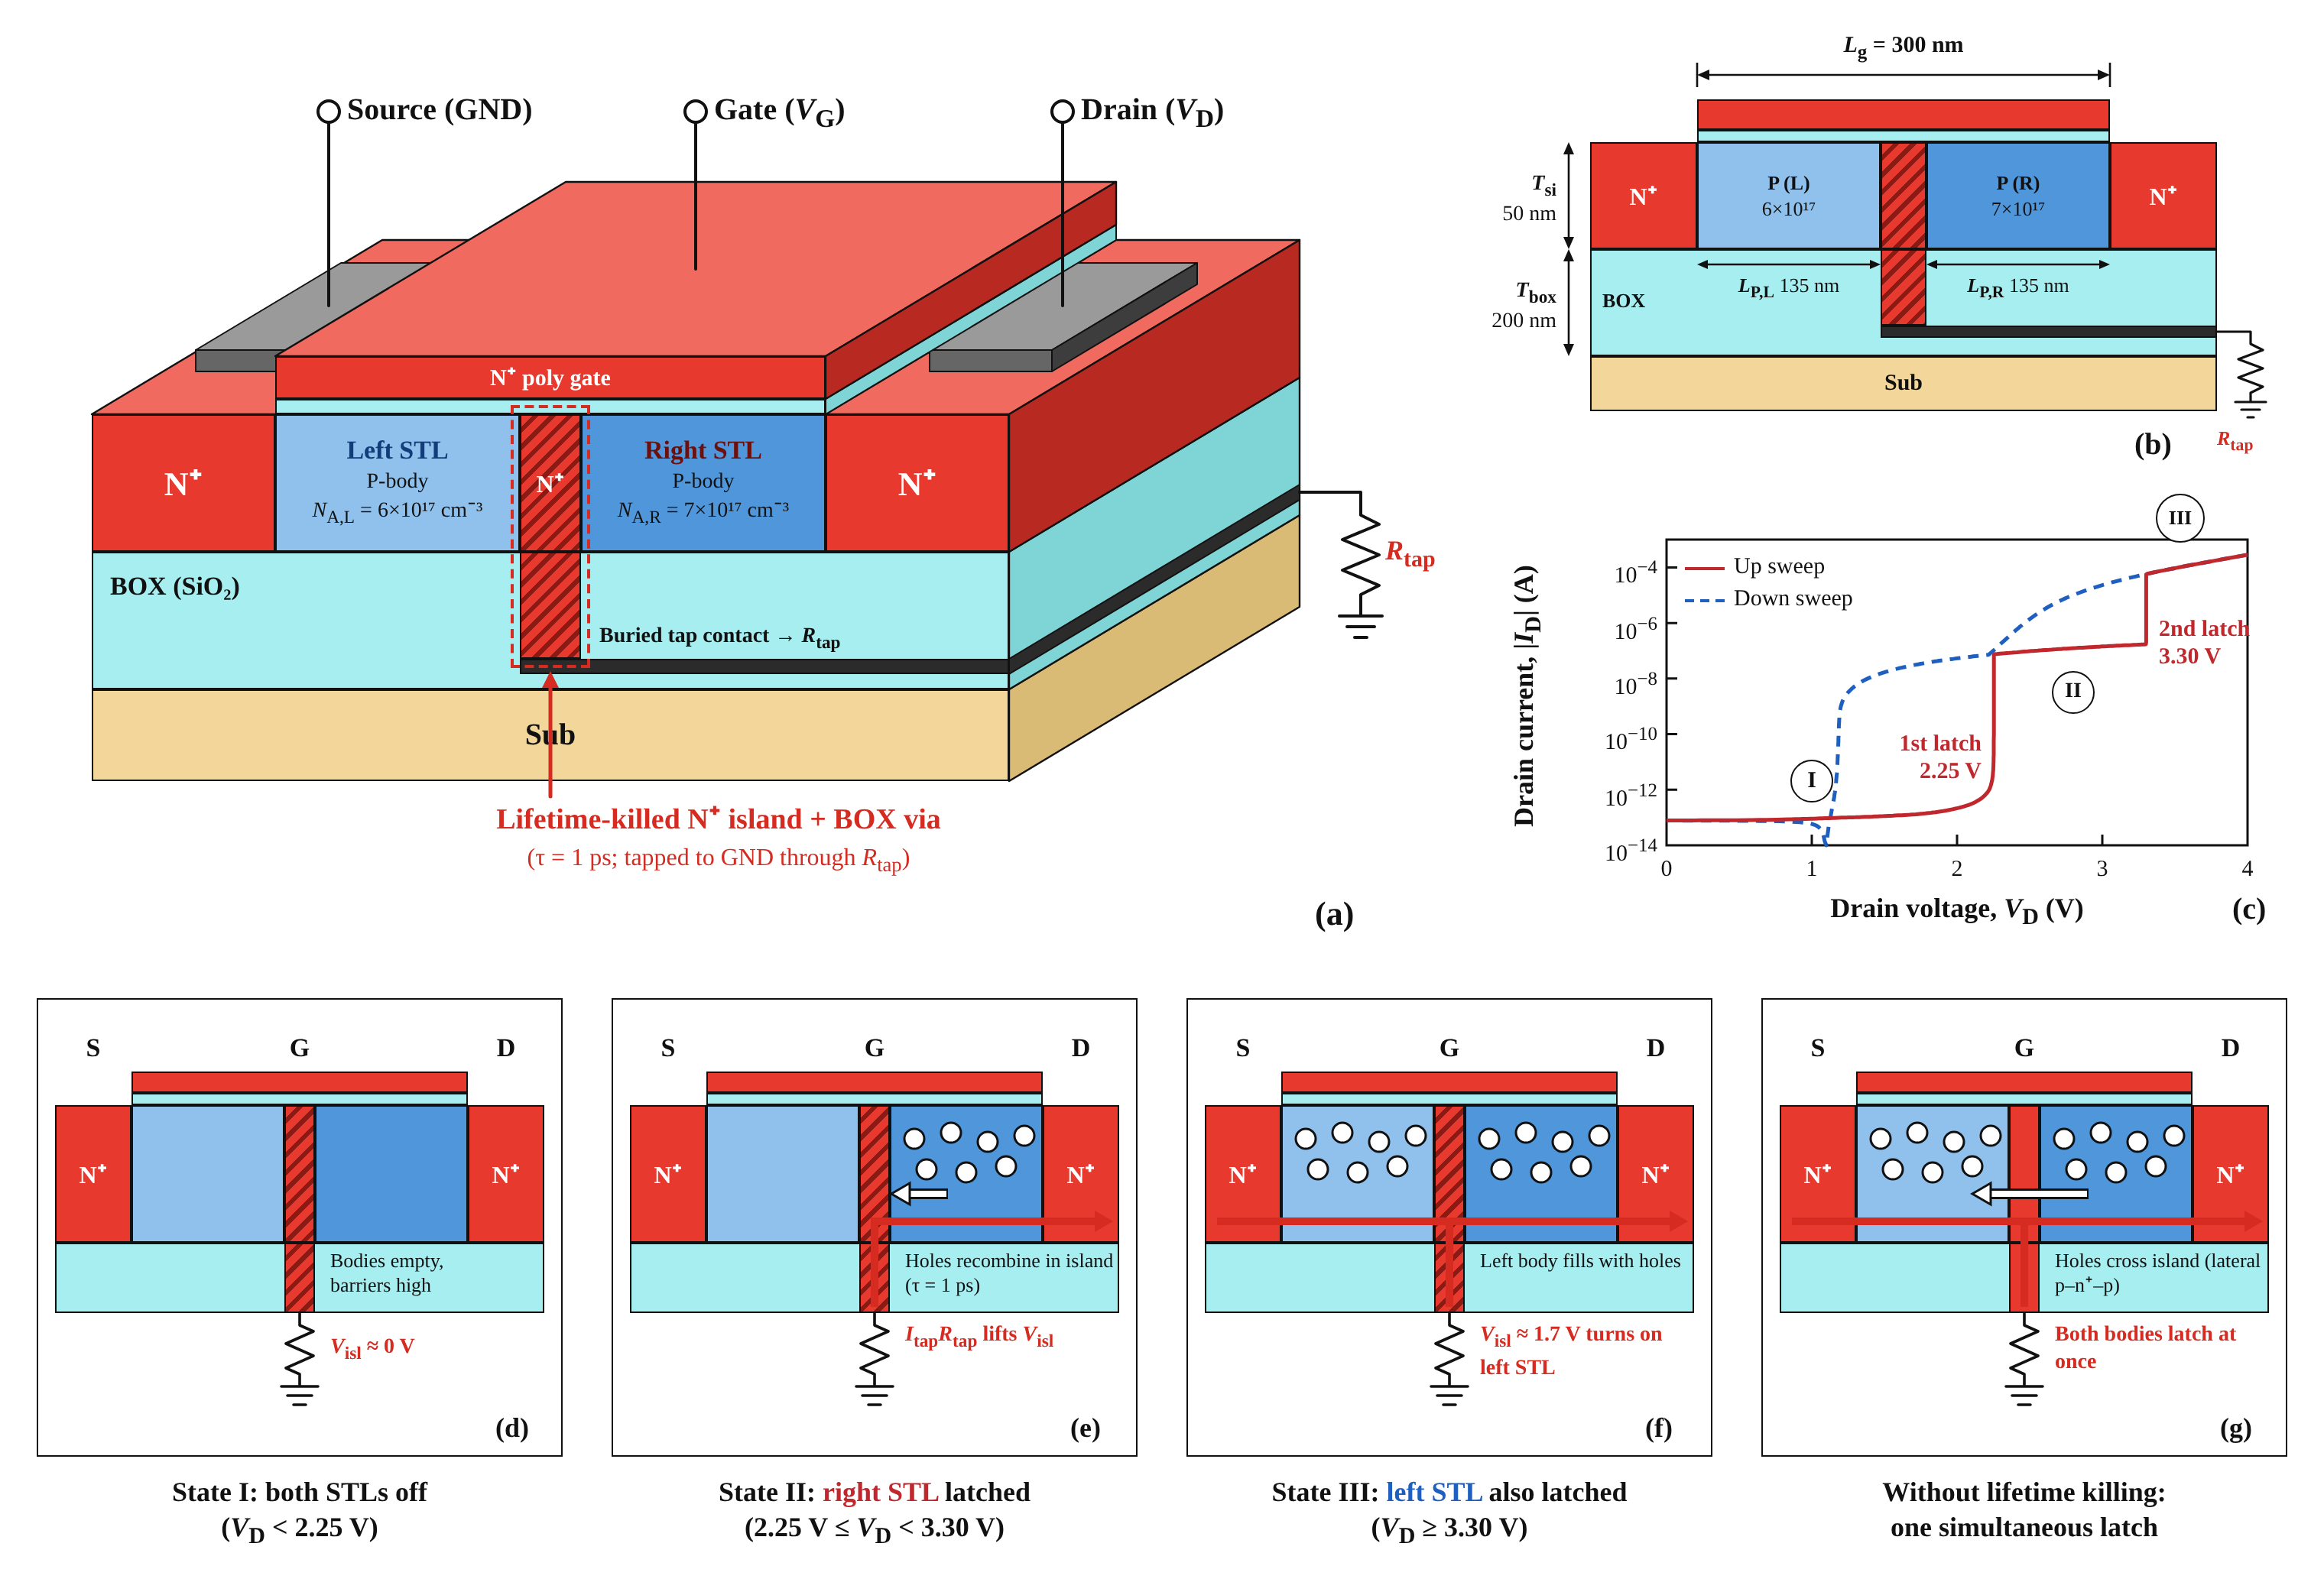
\includegraphics[width=\textwidth]{fig1_concept.png}
\caption{제안 소자와 동작 원리. (a) 왼쪽 STL(p-body $6\times10^{17}$)과 오른쪽 STL(p-body $7\times10^{17}$) 사이의 \textit{lifetime-killed} n$^+$ island를 BOX 관통 via와 $R_{tap}$으로 접지한다. (b) 단면과 치수. (c) Id-Vd의 두 래치(I$\rightarrow$II 2.25~V, II$\rightarrow$III 3.30~V). (d)--(f) 각 상태의 body 정공. (g) 섬 \textit{lifetime}을 줄이지 않으면 정공이 섬을 건너 두 body가 동시에 래치한다. 그림: \dpath{docs/fig/paper/fig1\_concept.png}; (c)의 데이터: \dpath{1007\_ddsplit/DDS\_BASE.log\_tr.log}.}
\label{fig:concept}
\end{figure*}

\section{소자 구조와 시뮬레이션 방법 (Device and Methodology)}
\subsection{기준 소자}
Table~\ref{tab:param}에 기준 소자 변수를 정리하였다. $L_g=300$~nm, $T_{si}=50$~nm, $t_{ox}=20$~nm, $T_{box}=200$~nm, S/D n$^+$ $10^{20}$~cm$^{-3}$이며, $V_G=-0.2$~V로 채널을 닫은 상태에서 drain 전압을 올린다. 채널 가운데 30~nm 폭 n$^+$ island가 body를 왼쪽 STL(source--island)과 오른쪽 STL(island--drain)로 나눈다. Island는 BOX를 관통하는 n$^+$ via로 바닥의 \textit{tap} 전극에 연결되고, 회로의 $R_{tap}$을 거쳐 접지된다. Island와 via의 \textit{carrier lifetime}은 $\tau_{isl}=1$~ps이다. 소자의 \texttt{.str}에서 직접 그린 구조는 저장소의 \dpath{docs/fig/struct\_14\_main\_L6.png}에 있다.

\begin{table}[!t]
\caption{기준 소자 변수 (덱: \dpath{1001/tap/MM\_TAPT\_ISL\_W30LK\_L6\_R7\_R1e7\_UD75S\_MF\_DD\_W05\_VGm0p2.in})}
\label{tab:param}
\centering\footnotesize
\begin{tabular}{@{}lll@{}}
\toprule
기호 & 의미 & 값 \\ \midrule
$L_g$, $L_{S/D}$ & gate 길이, S/D 길이 & 300, 500 nm \\
$T_{si}$, $t_{ox}$, $T_{box}$ & Si, gate oxide, BOX 두께 & 50, 20, 200 nm \\
$N_{A,L}$, $N_{A,R}$ & 왼쪽/오른쪽 p-body 도핑 & $6\times10^{17}$, $7\times10^{17}$ cm$^{-3}$ \\
$W_{IS}$, $N_{D,IS}$ & island 폭, 도핑 & 30 nm, $10^{20}$ cm$^{-3}$ \\
$\tau_{0,isl}$, $\tau_{0,Si}$ & island / Si SRH 기준값 $\tau_0$ & 1 ps, $10^{-7}$ s \\
$\tau_{eff}$ & 실효 SRH \textit{lifetime} (\texttt{consrh}) & island $5\times10^{-16}$ s, body 6.7--7.7 ns \\
$R_{tap}$ & island--GND 저항 & 10 M$\Omega$ \\
$V_G$, sweep & gate, drain ramp & $-0.2$ V, 0.7 V/ms \\
width & 소자 폭 & 0.5 $\mu$m \\ \bottomrule
\end{tabular}
\end{table}

\begin{figure}[!t]
\centering
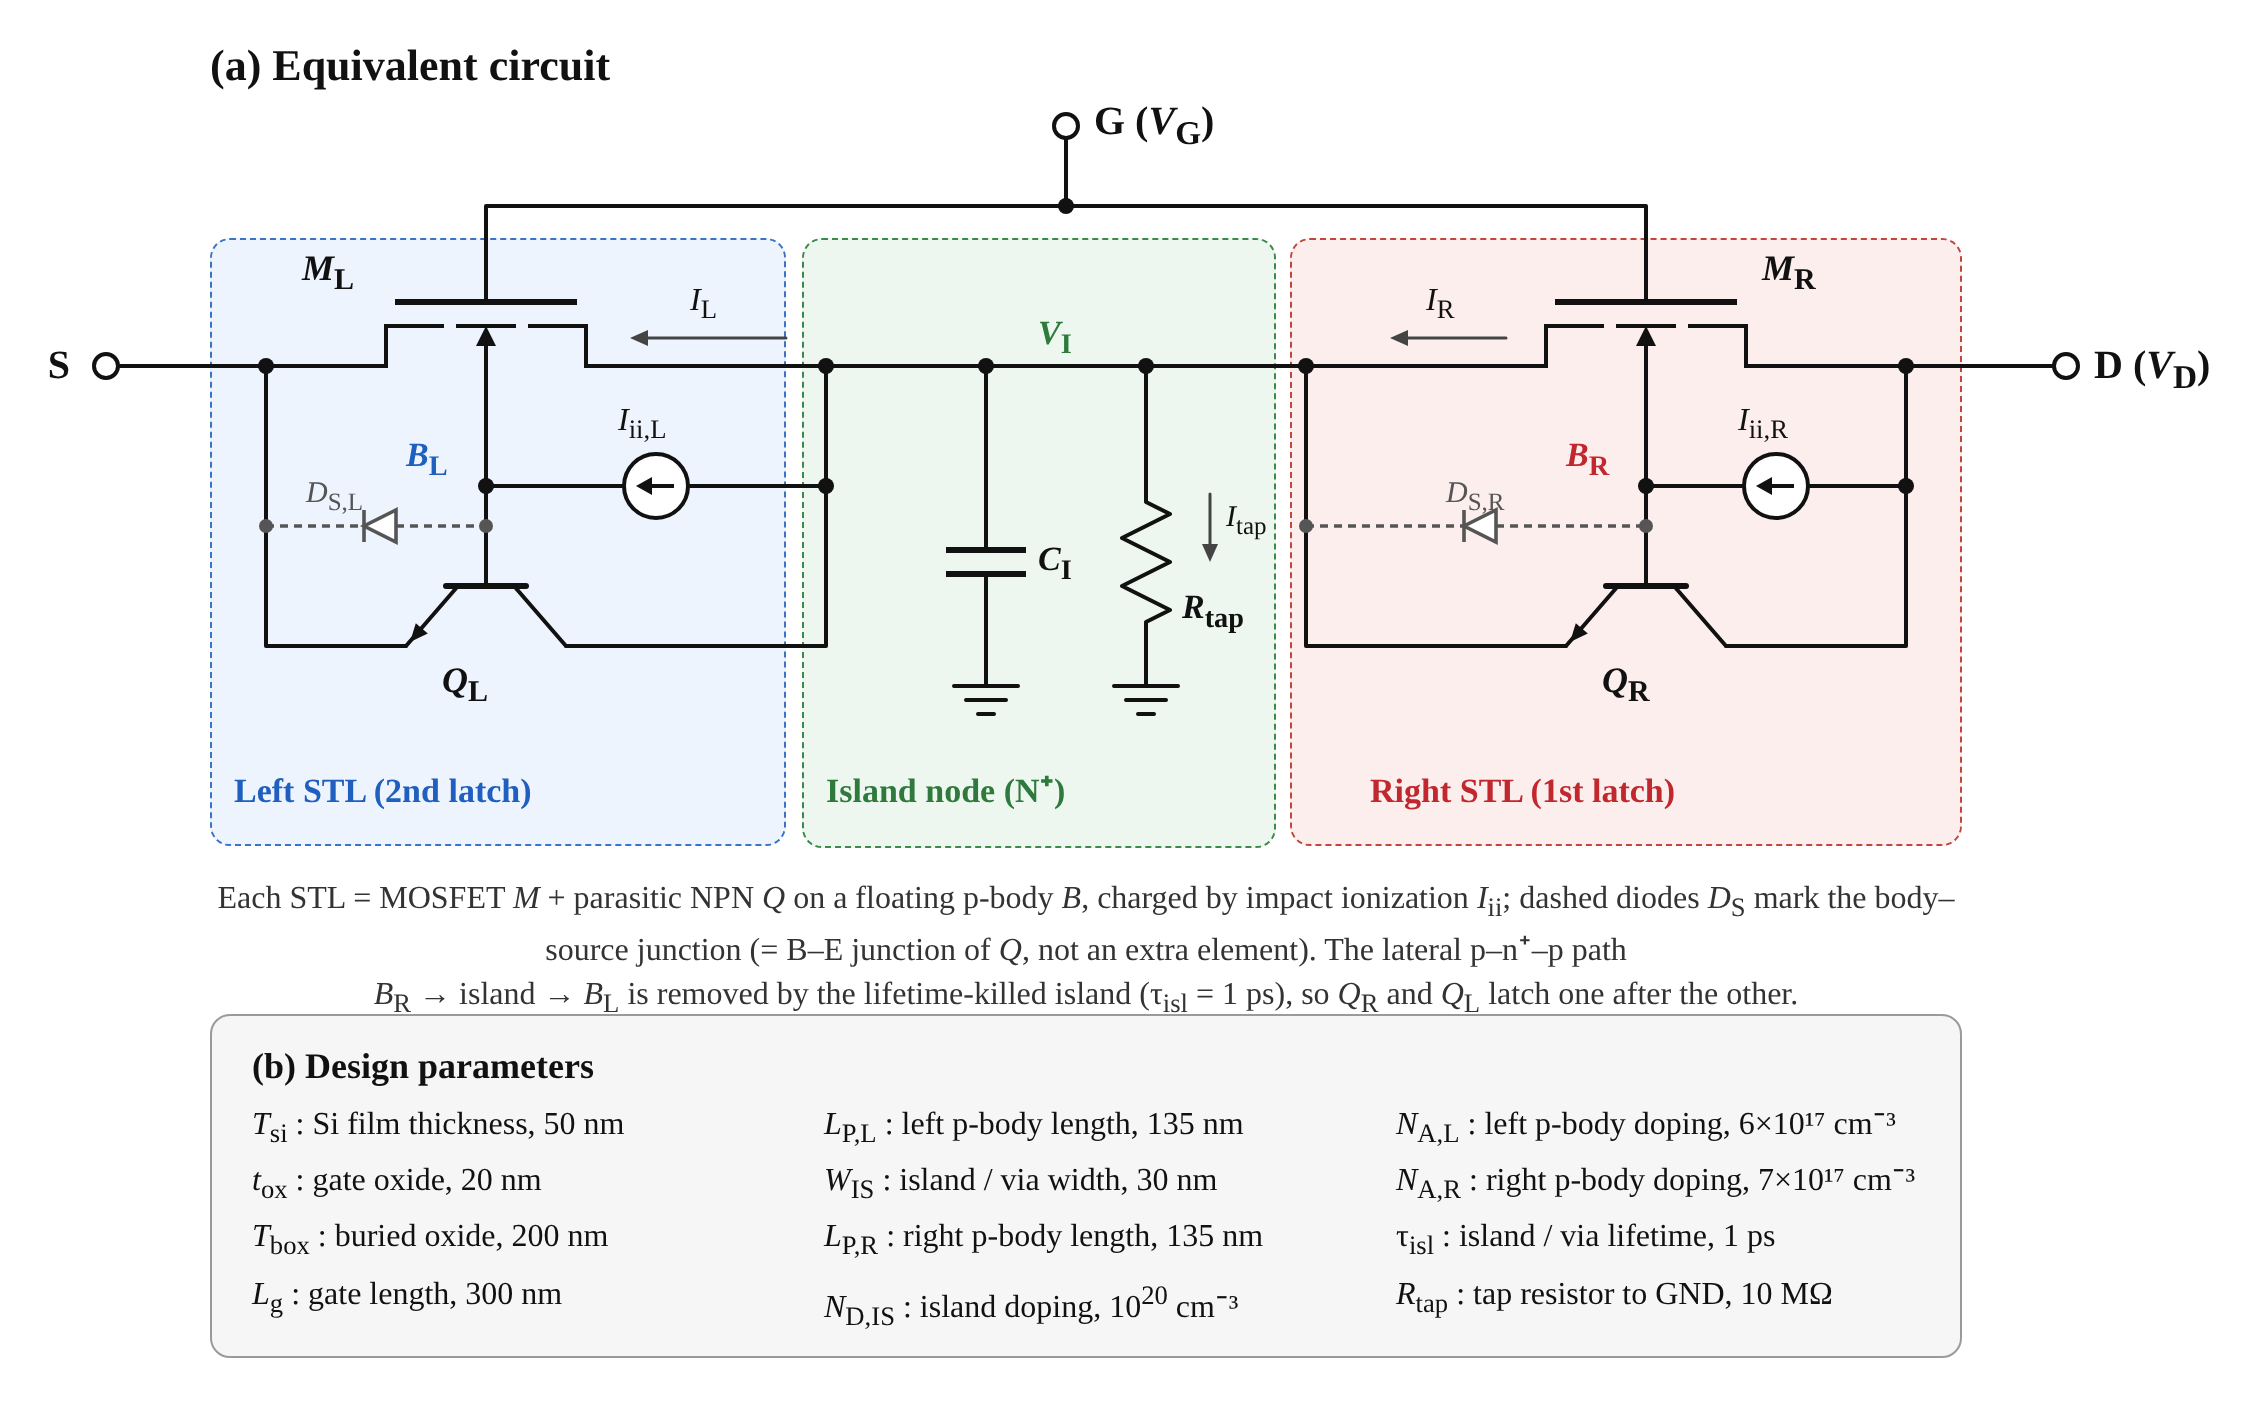
\includegraphics[width=\columnwidth]{fig2_equivalent_circuit.png}
\caption{(a) 등가 회로: 각 STL = MOSFET + floating body 위의 기생 NPN, \textit{impact ionization} 전류원 $I_{ii}$로 body가 충전된다. Island 노드 $V_I$는 $R_{tap}$으로 접지되어 오른쪽 STL의 source이자 왼쪽 STL의 drain이 된다. (b) 설계 변수. 그림: \dpath{docs/fig/paper/fig2\_equivalent\_circuit.png}.}
\label{fig:circuit}
\end{figure}

\subsection{물리 모델과 수치 방법}
모델은 \texttt{bgn}, \texttt{consrh}, \texttt{conmob}, \texttt{fldmob}, \texttt{fermi}, \texttt{trap.tunnel}, \texttt{bbt.std}와 Selberherr \textit{impact ionization} (\texttt{impact selb})~\cite{selberherr,maes}이다. \texttt{consrh}는 SRH \textit{lifetime}을 $\tau_{eff}=\tau_0/(1+N/N_{SRH})$, $N_{SRH}=5\times10^{16}$~cm$^{-3}$로 도핑에 따라 줄인다. 따라서 본문의 $\tau_{isl}$, $\tau_{Si}$는 모두 기준값 $\tau_0$이며, 실효값은 $10^{20}$~cm$^{-3}$ island에서 $\tau_0/2001$, $6$--$7\times10^{17}$ body에서 $\tau_0/13$--$\tau_0/15$이다. 기준 소자 \texttt{.str}에서 소수 캐리어 밀도와 재결합률로 구한 body 실효 \textit{lifetime}(켜진 오른쪽 body 6.2~ns)은 이 식과 일치하였다. Auger 재결합은 꺼져 있다. $10^{20}$~cm$^{-3}$에서 Auger \textit{lifetime}($\approx1/C_nN^2\approx0.4$~ns)은 island SRH 실효값보다 6자리 길고, body에서는 $\sim10^{-5}$~s이므로 결과에 미치는 영향은 작을 것으로 추정하며, Auger를 켠 확인 계산을 진행 중이다. 두 가지 \textit{transport}를 사용하였다: \textbf{에너지 균형(hcte)}과 \textbf{drift-diffusion (DD)}~\cite{atlas}. 래치는 S자 I--V(\textit{negative differential resistance})를 만들어 정상상태 전압 sweep이 접힘점에서 수렴하지 않는다. 그래서 drain을 0.7~V/ms로 올렸다 내리는 \textbf{transient ramp}를 사용하였다. 실제 시간 동역학이 불안정 가지를 건너가므로 래치와 \textit{hysteresis}가 바로 나온다. 10배 빠른 ramp(7~V/ms)에서는 래치 전압이 0.1~V 밀려 준정적이 아니므로 0.7~V/ms를 유지하였다. 최종 계산은 \textbf{MixedMode}로 하였다. 소자 구조와 $V_G$ 상태를 \texttt{.str}로 저장한 뒤 회로의 전압원, $R_{tap}$, (필요하면) drain 직렬 저항에 연결한다. MixedMode는 소자 단독 계산과 전류가 4자리까지 일치하면서 약 20배 빨랐다. 오른쪽 drain 접합은 1~nm 격자를 사용하였다.

\textbf{래치 판정.} 같은 인가 전압(2~mV 이내)에서 경로 전류가 1자리 넘게 변하고 실제 전류 수준(왼쪽 $|I_S|>10^{-7}$~A, 오른쪽 $|I_{tap}|>10^{-9}$~A)에 닿으면 래치로 정의하였다. 수치 오류와는 time step 붕괴, KCL 잔차, 내부 상태 변화, gate 변위전류로 구별하였다 (Section~VII).

\section{구조의 진화: 왜 래치가 한 번이었나}
이 절은 래치를 두 번 얻기까지 시도한 구조를 순서대로 기술한다. 각 단계는 \textbf{목적 $\rightarrow$ 방법 $\rightarrow$ 문제 $\rightarrow$ 해결}의 흐름을 따른다. 요약은 Fig.~\ref{fig:evol}, 각 단계의 상세 데이터는 Fig.~\ref{fig:doping}--\ref{fig:leftx}에 있다.

\begin{figure*}[!t]
\centering
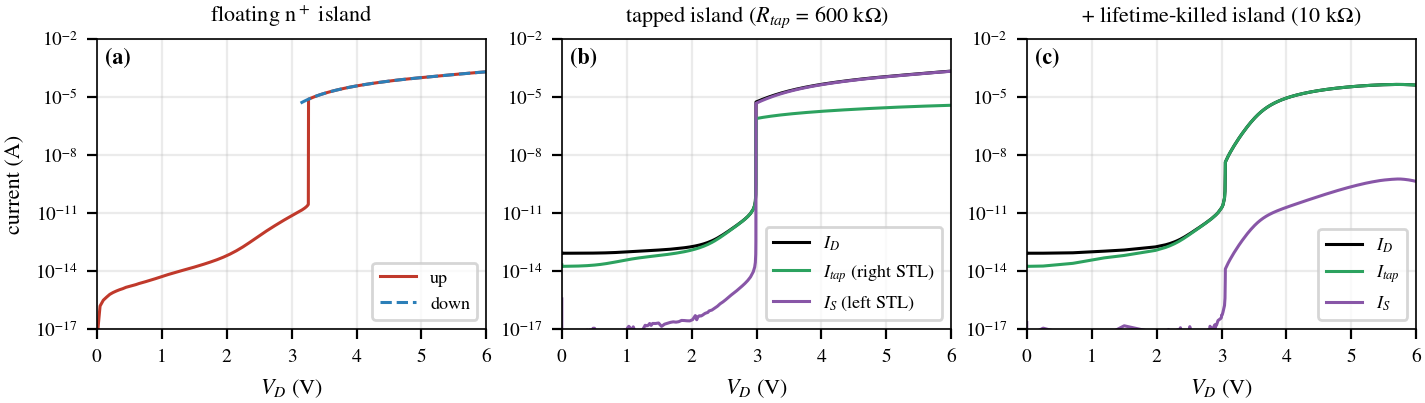
\includegraphics[width=0.9\textwidth]{fig3_evolution.png}
\caption{구조 변경에 따른 래치. (a) Floating n$^+$ island: 두 STL이 3.26~V에서 함께 래치. (b) $R_{tap}=600$~k$\Omega$로 접지한 island: 오른쪽($I_{tap}$)과 왼쪽($I_S$)이 2.99~V에서 동시에 점프(가로 PNP 결합). (c) Island \textit{lifetime} 1~ps: 오른쪽 STL만 래치하고 왼쪽은 꺼진 채 유지. 데이터: (a) \dpath{0928/ISL\_W30\_L3\_R7.log}, (b) \dpath{1001/tap/TAPT\_ISL\_W30\_L3\_R7\_R3e5\_VGm0p2.log}, (c) \dpath{1001/tap/TAPT\_ISL\_W30LK\_L3\_R7\_R1e4\_UD6S\_VGm0p2\_extract.dat}. 코드: \dpath{paper/make\_figs.py}.}
\label{fig:evol}
\end{figure*}

\subsection{Body 도핑 split}
\textbf{목적.} Body 왼쪽/오른쪽 도핑이 다르면 두 영역의 래치 전압이 달라 Id-Vd에 래치가 두 번 나올 것이라 기대하였다.
\textbf{방법.} 균일 $5\times10^{17}$ STL을 기준으로 (i) 소농도차 split(L/R $=4.8$--$5.4\times10^{17}$, 4--12\%), (ii) 대농도차 split(평균 약 $5\times10^{17}$, 비율 2.3/4/10배, 고도핑을 drain 쪽 또는 source 쪽)을 계산하였다.
\textbf{결과.} 모든 경우 래치가 \textbf{한 번}이었다 [Fig.~\ref{fig:doping}]. 소농도차는 균일 소자($V_{LU}=3.86$, $V_{LD}=3.51$~V)와 $\pm0.15$~V 이내로 같았다. 대농도차에서는 고도핑 방향과 비율이 래치 창을 조절하였다. Drain 쪽 고도핑(L3 R7)은 $V_{LU}=3.67$, 창 0.35~V로 균일 소자보다 낮아지고, source 쪽 고도핑은 L7 R3에서 4.89/3.88~V(창 1.01~V), L8 R2에서 5.76/4.11~V(창 1.66~V)로 올라갔다. L2 R8, L1 R10은 S자 I--V의 접힘점에서 전압 sweep이 3.5~V에서 멈추었고, L10 R1은 6.9~V까지 래치가 없었다.
\textbf{원인.} 전이 전후 EBD에서 \textit{hole quasi-Fermi level}이 body 전체에서 하나로 이어져 있었다. p/p$^+$ 계단은 다수 캐리어(정공)를 막지 못하므로 두 영역의 body 전위가 따로 움직일 수 없다. 또 저농도 쪽이 drain 쪽이면 공핍되어 정공 저장소가 하나만 남는다. 결론적으로 body를 \textbf{물리적으로} 나누어야 한다.

\begin{figure*}[!t]
\centering
\includegraphics[width=\textwidth]{figA_doping_split.pdf}
\caption{Body 도핑 split (단일 body, hcte, 전압 sweep). (a) 소농도차 split (단위 $10^{17}$~cm$^{-3}$, 실선 up, 점선 down): 균일 소자와 거의 같다. (b) 대농도차 split: 래치는 한 번이며 고도핑 방향이 $V_{LU}$를 움직인다. (c) $V_{LU}$, $V_{LD}$ ($|I_D|=10^{-8}$~A 기준; L2 R8, L1 R10은 3.5~V에서 sweep 정지). 데이터: \dpath{0921/STL\_NB5p0\_localfine.log}, \dpath{0921/SPLIT\_*\_X50.log}, \dpath{0927/BIG\_\{L3\_R7,L7\_R3,L8\_R2,L10\_R1\}\_X50.log}, \dpath{0927\_bigsplit/BIG\_\{L2\_R8,L1\_R10\}\_X50.log}. 코드: \dpath{paper/make\_figs\_ext.py}.}
\label{fig:doping}
\end{figure*}

\subsection{단일 body의 다른 분리 시도}
도핑 외의 방법으로 두 body를 독립시킬 수 있는지 확인하였다 [Fig.~\ref{fig:single}]. (a) Body 아래쪽에 산화막 \textit{notch}(폭 10--20~nm)를 넣어 두 정공 저장소를 나누고, 위쪽 얇은 Si \textit{bridge}(두께 5--20~nm)로 전자 경로만 남겼다. 래치는 한 번($V_{LU}=4.27$--4.44~V)이며, bridge가 얇을수록 래치가 약해져 B05 W10은 연속적으로 켜졌다. (b) Si 두께를 좌우로 나눈 $T_{si}$ split(20--50~nm)도 래치가 한 번이고 $V_{LU}$가 3.8--4.1~V 사이에서만 움직였다. (c) Gate를 둘로 나눈 \textit{split gate}에서는 두 번째 gate 전압 $V_{G2}$가 래치 창을 0.36에서 1.18~V로 조절하였으나 역시 한 번이었다. (d) Source 쪽(S) 또는 drain 쪽(D)에 gate로 제어되는 n$^{-}$ 영역(75--150~nm)을 둔 n$^+$/n$^-$/p/n$^+$ 구조는 n$^-$ 장벽 붕괴가 래치와 별개의 단계로 나타나기를 기대하였으나, 래치는 한 번(2.4--3.2~V)이었다. 같은 시기 Id-Vg [Fig.~\ref{fig:idvg}]에서는 drain 쪽 고도핑(L3 R7)만 $V_D=1$~V에서 gate 방향 래치(up 1.390/down 1.335~V)를 보였고, 다른 도핑 배치는 연속적이었다.

\begin{figure*}[!t]
\centering
\includegraphics[width=\textwidth]{figB_single_body.pdf}
\caption{단일 body에서의 다른 분리 시도 (모두 래치 한 번). (a) 산화막 notch + Si bridge (B: bridge 두께, W: notch 폭, nm). (b) $T_{si}$ split (왼쪽/오른쪽 두께 nm). (c) Split gate: 두 번째 gate 전압 $V_{G2}$ (D: drain 쪽, S: source 쪽 gate). (d) n$^+$/n$^-$/p/n$^+$ (S/D: n$^-$ 위치, Ln: n$^-$ 길이 nm, N: n$^-$ 도핑, P: p 도핑). 데이터: \dpath{0921/B*\_W*\_L5p0\_R5p2.log}, \dpath{0928/TSI\_*.log}, \dpath{0929/splitgate/SG\_*.log}, \dpath{1001/nnpn/NNPN\_*.log}.}
\label{fig:single}
\end{figure*}

\begin{figure}[!t]
\centering
\includegraphics[width=\columnwidth]{figC_idvg.pdf}
\caption{대농도차 split의 Id-Vg. (a) $V_D=0.05$~V(점선)와 1~V(실선). (b) $V_D=1$~V gate 왕복: L3 R7만 1.39/1.34~V의 gate 방향 래치와 \textit{hysteresis}를 보인다. 데이터: \dpath{0928/idvg/IDVG\_BIG\_*\_X50\_\{vd0p05,vd1\}.log}, \dpath{0928/idvg\_return/IDVGR\_BIG\_*\_X50\_vd1.log}.}
\label{fig:idvg}
\end{figure}

\subsection{Floating n$^+$ island: 직렬 제약}
\textbf{목적.} 정공이 두 body 사이를 오가지 못하게 하면 두 body가 따로 래치할 것이다.
\textbf{방법.} 채널 가운데에 폭 30~nm, $10^{20}$~cm$^{-3}$의 n$^+$ island를 Si 두께 전체에 넣어 왼쪽 STL(source--island)과 오른쪽 STL(island--drain)을 만들었다.
\textbf{결과.} 래치 전 두 body 전위는 $-0.02$와 0.36~V로 달라 분리 자체는 되었다 [Fig.~\ref{fig:island}(b)]. 그러나 L3 R7에서 3.26~V에 왼쪽 body, 오른쪽 body, island가 \textbf{동시에} 점프하였다. L5 R5, L7 R3은 sweep이 4.9--5.4~V에서 멈추었다.
\textbf{원인.} 섬이 떠 있으면 오른쪽 STL의 전류가 반드시 왼쪽 STL을 지나야 한다(\textbf{직렬 제약}). 따라서 한쪽만 켜질 수 없다. 섬에 따로 빠져나갈 전류 경로가 필요하다.

\begin{figure}[!t]
\centering
\includegraphics[width=\columnwidth]{figD_island.pdf}
\caption{Floating n$^+$ island (폭 30~nm). (a) 도핑 배치별 $|I_D|$. (b) L3 R7의 probe 전위: 래치 전에는 두 body가 다른 전위이지만 3.26~V에서 함께 점프한다. 데이터: \dpath{0928/ISL\_W30\_\{L3\_R7,L5\_R5,L7\_R3\}.log}.}
\label{fig:island}
\end{figure}

\subsection{Tapped island: transient ramp와 가로 PNP 결합}
\textbf{목적.} 섬을 저항 $R_{tap}$으로 접지하면 오른쪽 STL이 먼저 켜졌을 때 그 전류가 왼쪽을 거치지 않고 빠진다. 섬 전위 $I_{tap}R_{tap}$은 왼쪽 STL의 drain 전압이 되어 두 번째 래치를 일으킬 것이다.
\textbf{방법.} 섬 아래 BOX를 n$^+$ via로 관통시키고 바닥 \textit{tap} 전극에 \texttt{contact resistance}를 달았다.
\textbf{문제 1: 접힘점 수렴.} 전압 sweep은 2.93~V, $1.6\times10^{-11}$~A에서 멈추었다. Drain 직렬 저항($10^5$~$\Omega$), 전류 sweep, 전압--전류 제어 전환도 모두 래치 전에 멈추었다 (Table~\ref{tab:conv}). Drain을 시간에 대해 0.7~V/ms로 올리는 \textbf{transient ramp}만이 0--7--0~V를 완주하였다. 실제 시간 동역학이 불안정 가지를 건너가므로 점프와 \textit{hysteresis}가 바로 얻어진다. 이후 모든 계산은 이 방식이다.
\textbf{문제 2: 동시 래치.} $R_{tap}$을 600, 60, 10~k$\Omega$로 바꿔도 $V_{LU}$는 모두 2.990~V였다 [Fig.~\ref{fig:tap}(a)]. 섬 전위는 래치 후 $R_{tap}$에 비례하여 올랐지만 [Fig.~\ref{fig:tap}(b)], 점프 순간을 확대하면 [Fig.~\ref{fig:tap}(c)] 오른쪽 body가 먼저 오르고 약 10~ns 뒤 왼쪽 body와 섬이 따라 올라 \textbf{한 번의 점프 안의 순서}에 불과하였다.
\textbf{원인.} 오른쪽 p body--n$^+$ island(30~nm)--왼쪽 p body가 \textbf{가로 PNP}를 이룬다. 오른쪽에서 섬으로 들어간 정공이 얇은 섬을 재결합 없이 건너 왼쪽 body를 채운다.

\begin{table}[!t]
\caption{S자 I--V 접힘점에서의 계산 방법 비교 ($R_{tap}=600$~k$\Omega$; 덱: \dpath{1001/tap/TAP*\_ISL\_W30\_L3\_R7\_*.in})}
\label{tab:conv}
\centering\footnotesize
\begin{tabular}{@{}p{0.42\columnwidth}p{0.5\columnwidth}@{}}
\toprule
방법 & 결과 \\ \midrule
전압 sweep & 2.934~V, $1.65\times10^{-11}$~A에서 정지 \\
drain 직렬 $10^5$~$\Omega$ & 효과 없음 (pA에서 $IR\approx0$) \\
전류 sweep & $2.3\times10^{-15}$~A (0.69~V)에서 실패 \\
전압$\rightarrow$전류 제어 & $4.3\times10^{-11}$~A에서 정지 \\
\textbf{transient ramp 0.7~V/ms} & \textbf{0$\rightarrow$7$\rightarrow$0~V 완주} \\ \bottomrule
\end{tabular}
\end{table}

\begin{figure*}[!t]
\centering
\includegraphics[width=\textwidth]{figE_tap.pdf}
\caption{Tapped island (섬 \textit{lifetime} 기본값, transient ramp). (a) $R_{tap}$ 600/60/10~k$\Omega$: 모두 2.990~V에서 래치. (b) 섬 전위 상승: $R_{tap}$이 클수록 크다. (c) $R_{tap}=600$~k$\Omega$ 점프 부근 확대: 오른쪽 body가 먼저, 약 10~ns 뒤 왼쪽 body와 섬이 따라온다(가로 PNP 결합). 데이터: \dpath{1001/tap/TAPT\_ISL\_W30\_L3\_R7\_\{R3e5,R3e4\}\_VGm0p2.log}, \dpath{1001/tap/TAPT\_ISL\_W30\_L3\_R7\_R1e4\_UP\_VGm0p2.log}.}
\label{fig:tap}
\end{figure*}

\subsection{가로 PNP 결합 끊기: 섬 폭, top contact, lifetime}
\textbf{목적.} 정공이 섬을 건너지 못하게 하면 오른쪽 STL만 혼자 래치할 것이다.
\textbf{방법.} $R_{tap}=10$~k$\Omega$에서 세 가지를 비교하였다: 섬 폭 30$\rightarrow$100~nm (W100), 섬 윗면 \textit{ohmic contact}로 tap (C), 섬과 via의 SRH \textit{lifetime}을 1~ps로 줄인 섬 (B).
\textbf{결과} [Fig.~\ref{fig:decouple}]. W100은 1.66~V에서 서서히 켜지고, $V_G$를 $-1.2$~V까지 내려도 $I_S$가 $I_D$를 따라왔다. 정공이 100~nm 섬도 건넌다. C는 3.035~V에서 $I_{tap}$과 $I_S$가 함께 점프하였다. 정공이 5~nm 깊이 contact 아래로 지나가기 때문이다. \textbf{B만} 3.058~V에서 오른쪽 STL($I_{tap}$)이 혼자 래치하고 $I_S\le5.4\times10^{-10}$~A로 왼쪽이 꺼진 채 남았다. B는 0--6--0~V 왕복에서 같은 3.0~V에 꺼진 상태(up)와 켜진 상태(down)가 공존하는 쌍안정 동작을 보였다.
\textbf{문제.} 분리는 되었지만 왼쪽 STL이 구동되지 않았다. $R_{tap}=10$~k$\Omega$에서 섬 전위가 0.4~V 이상 오르지 않는다.

\begin{figure*}[!t]
\centering
\includegraphics[width=\textwidth]{figF_decouple.pdf}
\caption{가로 PNP 결합을 끊는 세 방법 ($R_{tap}=10$~k$\Omega$). (a) 섬 폭 100~nm, $V_G=-0.2/-0.5/-1.2$~V (실선 $I_D$, 점선 $I_S$): 왼쪽이 함께 켜진다. (b) 섬 윗면 ohmic contact(C): $I_{tap}$, $I_S$가 동시에 점프. (c) 섬 \textit{lifetime} 1~ps(B): 오른쪽만 래치하고 $I_S$는 $10^{-9}$~A 아래 (점선 down). 데이터: \dpath{1001/tap/TAPT\_ISL\_W100\_L3\_R7\_R1e4\_\{UP\_VGm0p2,UPDN\_VGm0p5,UPDN\_VGm1p2\}.log}, \dpath{1001/tap/TAPT\_ISL\_W30TC\_L3\_R7\_R1e4\_UD6S\_VGm0p2.log}, \dpath{1001/tap/TAPT\_ISL\_W30LK\_L3\_R7\_R1e4\_UD6S\_VGm0p2\_extract.dat}.}
\label{fig:decouple}
\end{figure*}

\subsection{섬 전위 올리기: $R_{tap}$}
B 구조에서 $R_{tap}$을 10~k, 300~k, 1~M$\Omega$로 키웠다 [Fig.~\ref{fig:BR}]. $V_D=4.98$~V에서 오른쪽 $I_D$는 $3.2\times10^{-5}$, $3.2\times10^{-6}$, $1.1\times10^{-6}$~A로 줄고, 섬 전위 상승은 0.32, 0.94, 1.05~V, 왼쪽 $I_S$는 $2.1\times10^{-10}$, $3.3\times10^{-8}$, $7.3\times10^{-8}$~A로 늘었다. 섬 전위는 $V_D$ 1~V당 약 0.73~V씩 오르고 $I_S$는 지수적으로 커졌다. 그러나 왼쪽 도핑 $3\times10^{17}$에서는 $I_S$가 \textbf{점프 없이 매끄럽게} 올랐고, $R_{tap}=1$~M$\Omega$ run은 5.284~V에서 멈추었다. 직전의 음전류 점프는 수치 오류였다 (Section~VII).

\begin{figure}[!t]
\centering
\includegraphics[width=\columnwidth]{figG_B_R.pdf}
\caption{B 구조(섬 \textit{lifetime} 1~ps)에서 $R_{tap}$ sweep (up). (a) 왼쪽 STL 전류 $|I_S|$, (b) 섬 전위 상승. 1~M$\Omega$ 곡선은 5.28~V의 수치 오류 직전까지 표시. 데이터: \dpath{1001/tap/TAPT\_ISL\_W30LK\_L3\_R7\_\{R1e4\_UD6S,R3e5\_UD7S\}\_VGm0p2\_extract.dat}, \dpath{1001/tap/TAPT\_ISL\_W30LK\_L3\_R7\_R1e6\_UD7S\_VGm0p2.log}.}
\label{fig:BR}
\end{figure}

\subsection{왼쪽 STL은 래치할 수 있는가: standalone 소자}

섬부터 오른쪽을 모두 n$^+$로 바꾼 \textbf{standalone 왼쪽 STL}(body 135~nm)로 도핑을 탐색하였다 [Fig.~\ref{fig:left}]. 이 소자의 $V_D$는 본 소자에서 왼쪽 래치에 필요한 섬 전위에 해당한다. 원래 왼쪽 도핑 $3\times10^{17}$과 $5\times10^{17}$은 장벽이 낮아 \textbf{연속적으로 켜졌고} 래치가 없었다. $6\times10^{17}$부터 급격한 래치가 생겼다 (hcte: 2.54~V, \textit{hysteresis} 2.48--2.32~V; DD: 1.78~V). B 소자 안의 왼쪽 STL 전류는 standalone 곡선과 2--3배 이내로 일치하여, standalone 소자가 대표성이 있음을 확인하였다. 이로써 왼쪽 body를 $6\times10^{17}$으로 정하였다. $6\times10^{17}$은 0--3--0~V 왕복에서 켜짐 2.541~V, 꺼짐 2.48--2.32~V의 \textit{hysteresis}를 가지며, 같은 2.4~V에서 꺼진 상태와 켜진 상태의 장벽 높이가 달랐다. Ramp를 7~V/ms로 10배 빠르게 하면 $V_{LU}$가 2.645~V로 0.1~V 밀리고 꺼짐은 같았다 [Fig.~\ref{fig:leftx}(b),(c)]. 래치 직전 body 전위 VB$_{left}$는 0.25~V 부근에서 급격히 0.45~V로 뛰며, 이는 body--source 접합이 순방향으로 바뀌는 순간이다. 따라서 0.7~V/ms를 준정적 조건으로 유지하였다. Fig.~\ref{fig:leftx}(a)는 B 소자($R_{tap}=300$~k$\Omega$) 안의 왼쪽 STL 전류를 섬 전위 상승에 대해 그린 것으로, 같은 도핑의 standalone 곡선과 2--3배 이내로 겹친다.

\begin{figure}[!t]
\centering
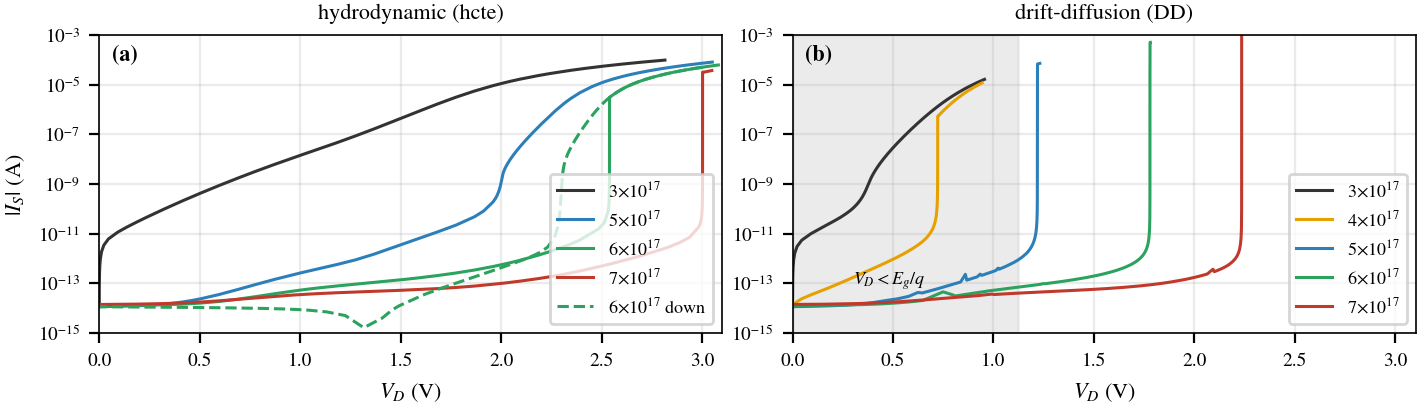
\includegraphics[width=\columnwidth]{fig4_left_stl.png}
\caption{Standalone 왼쪽 STL의 source 전류. (a) hcte: $3\times10^{17}$, $5\times10^{17}$은 연속적으로 켜지고, $6\times10^{17}$($V_{LU}=2.54$~V, 점선: down sweep)과 $7\times10^{17}$(3.00~V)은 급격히 래치한다. (b) DD: 래치 전압이 0.7--0.8~V 낮고, $V_D<E_g/q$ 영역의 래치(회색)는 DD의 \textit{impact ionization} 과대평가로 본다. 데이터: \dpath{1001/tap/LEFTONLY\_L135\_P\{3,5,6,7\}e17\_UD6S\_VGm0p2.log}, \dpath{1001/tap/LEFTONLY\_L135\_P6e17\_UD3\_VGm0p2.log}, \dpath{1001/tap/LEFTONLY\_L135\_P*\_DD\_UP4\_VGm0p2.log}.}
\label{fig:left}
\end{figure}

\begin{figure*}[!t]
\centering
\includegraphics[width=\textwidth]{figH_left_extra.pdf}
\caption{Standalone 왼쪽 STL의 검증. (a) B 소자 안의 왼쪽 STL ($I_S$ vs 섬 전위 상승, $R_{tap}=300$~k$\Omega$)과 standalone 소자 ($I_S$ vs $V_D$), 둘 다 $3\times10^{17}$. (b) $6\times10^{17}$ 왕복의 ramp 속도 비교 (실선 up, 점선 down). (c) 같은 run의 왼쪽 body probe 전위. 데이터: \dpath{1001/tap/LEFTONLY\_L135\_P3e17\_UD6S\_VGm0p2.log}, \dpath{1001/tap/TAPT\_ISL\_W30LK\_L3\_R7\_R3e5\_UD7S\_VGm0p2\_extract.dat}, \dpath{1001/tap/LEFTONLY\_L135\_P6e17\_\{UD3,UD3\_R7\}\_VGm0p2.log}.}
\label{fig:leftx}
\end{figure*}

\section{두 단계 래치 (Two-Stage Latch)}
최종 소자[$N_{A,L}=6\times10^{17}$, $R_{tap}=10$~M$\Omega$, Table~\ref{tab:param}]의 DD MixedMode 결과가 Fig.~\ref{fig:dl}이다. 올라갈 때 \textbf{2.251~V}에서 오른쪽 STL이 래치하여 $I_{tap}$이 $10^{-12}$에서 $7\times10^{-8}$~A로 뛰고(상태 I$\rightarrow$II), 섬 전압 $V_{tap}$이 0.75~V로 오른다. 이후 $V_{tap}$이 $V_D$를 따라 오르다가 1.67~V에 이르는 \textbf{3.300~V}에서 왼쪽 STL이 래치한다(II$\rightarrow$III). 이 섬 전압은 standalone 왼쪽 STL의 DD $V_{LU}$(1.78~V)와 가깝다. 두 번째 래치에서 $I_S$는 같은 $V_D$에서 약 1~$\mu$s 안에 $3\times10^{-7}$에서 $5\times10^{-5}$~A로 뛰고, 전류가 왼쪽 STL로 직접 흐르면서 $V_{tap}$이 1.24~V로 떨어진다. 내려올 때 왼쪽은 약 2.24~V, 오른쪽은 약 1.20~V에서 꺼져 \textbf{두 래치 모두 \textit{hysteresis}}를 가진다.

이 두 번째 점프는 수치 오류가 아니다. 점프 동안 time step은 $10^{-10}$~s 수준으로 과정을 따라가고, KCL 잔차는 $10^{-15}$~A 이하이다. 점프 후 전류는 일정 값에 안정되며, 점프 직전에는 $I_S$의 기울기가 커지는 양의 되먹임 전조가 있다. 소자 폭을 1~$\mu$m로 계산한 첫 run과 0.5~$\mu$m run의 래치 전압 차이는 6~mV 이내였다.

\begin{figure*}[!t]
\centering
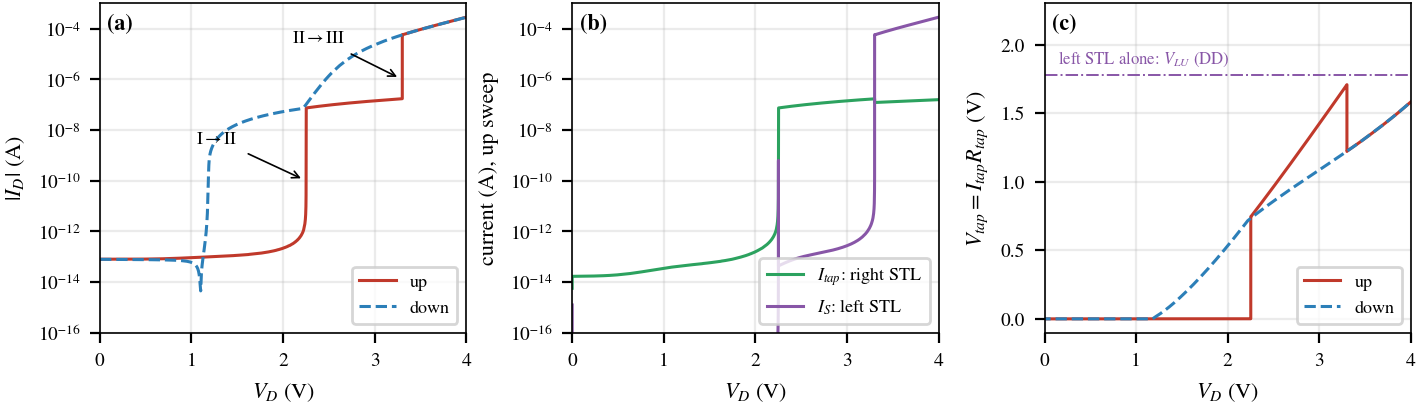
\includegraphics[width=0.9\textwidth]{fig5_double_latch.png}
\caption{두 단계 래치 (DD, MixedMode, $R_{tap}=10$~M$\Omega$, 폭 0.5~$\mu$m). (a) $|I_D|$--$V_D$ (실선 up, 점선 down): 2.251~V와 3.300~V의 두 래치와 각각의 \textit{hysteresis}. (b) 경로별 전류: 오른쪽 STL($I_{tap}$)이 먼저, 왼쪽 STL($I_S$)이 다음에 래치. (c) 섬(tap) 전압: 왼쪽 STL의 drain 전압으로 작용하여 standalone $V_{LU}$ 부근에서 두 번째 래치를 일으킨다. 데이터: \dpath{1007\_ddsplit/DDS\_BASE.log\_tr.log} (같은 소자의 0--7.5--0~V run: \dpath{1001/tap/MM\_TAPT\_ISL\_W30LK\_L6\_R7\_R1e7\_UD75S\_MF\_DD\_W05\_VGm0p2.log\_tr.log}).}
\label{fig:dl}
\end{figure*}

\section{메커니즘: \texttt{.str} 기반 Hole Balance}
래치 전후에 촘촘히 저장한 \texttt{.str} 스냅샷 28개로 STL별 물리량을 계산하였다. 각 STL에 대해 (i) source--body 전자 장벽, (ii) body 평균 정공 밀도, (iii) drain 쪽 최대 전계, (iv) \textit{impact ionization} 정공 전류 $I_{ii}=qW\!\int G_{ii}\,dA$, (v) body와 그 STL의 n$^+$ source(왼쪽: S, 오른쪽: island)에서의 재결합 전류를 구했다 (Si 삼각형 면적 적분).

\textbf{첫 번째 래치.} 2.24~V에서 오른쪽 drain 접합 전계는 $1.16\times10^6$~V/cm, 증배 $M-1=I_{ii}/I_e\approx0.25$이다. 정공이 오른쪽 body를 순방향으로 만들면 섬에서 전자 주입이 늘고 $I_{ii}$가 다시 늘어난다. 2.24$\rightarrow$2.26~V(20~mV)에서 $I_{ii}$가 $5\times10^{-13}$에서 $9\times10^{-9}$~A로 4자리 뛰고 장벽이 0.60에서 0.28~eV로 무너진다 [Fig.~\ref{fig:mech}(a),(b)]. 래치 후에는 $I_{ii}$가 body 재결합과 island 재결합의 합과 같다. 예를 들어 3.0~V에서 $1.96\times10^{-8}\approx1.06\times10^{-8}+1.00\times10^{-8}$~A이다.

\textbf{두 번째 래치.} 오른쪽이 켜진 뒤 섬 전위가 오르면 왼쪽 STL의 drain 쪽(섬 왼쪽 가장자리) 전계가 $3.6\times10^5$에서 $7.1\times10^5$~V/cm로 커진다(2.2$\rightarrow$3.28~V). 3.28$\rightarrow$3.32~V에서 왼쪽 장벽이 0.61에서 0.10~eV로 무너지고 $I_{ii}$가 $4\times10^{-13}$에서 $3.4\times10^{-6}$~A로 뛴다. Fig.~\ref{fig:mech}(c)의 $G_{ii}$ 지도에서 정공 생성이 두 drain 쪽 접합(섬 왼쪽 가장자리와 drain)에 모여 있다. 오른쪽에서 생긴 정공은 1~ps 섬에서 재결합하므로, 왼쪽은 \textbf{자기 drain 전계로만} 켜진다. 이것이 두 래치가 분리되는 이유이다.

\begin{figure*}[!t]
\centering
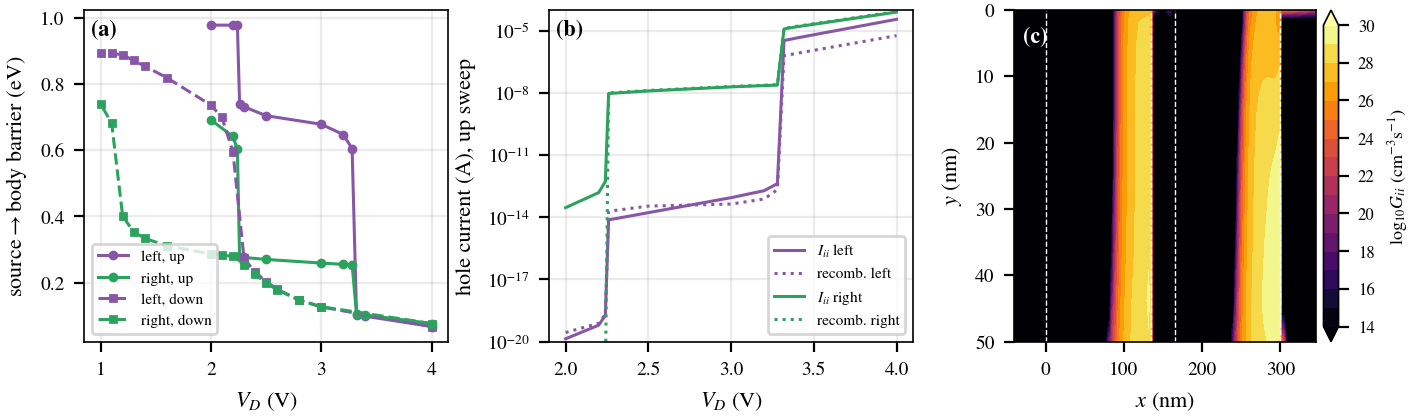
\includegraphics[width=0.9\textwidth]{fig6_mechanism.png}
\caption{\texttt{.str} 스냅샷 기반 메커니즘 (기준 소자, $\tau_{Si}=10^{-7}$~s). (a) STL별 source$\rightarrow$body 전자 장벽 (up 실선, down 점선): 각 래치에서 해당 STL의 장벽만 무너진다. (b) Up sweep의 \textit{impact ionization} 정공 전류(실선)와 재결합(점선). (c) 두 번째 래치 직후(3.32~V)의 $G_{ii}$ 2D 지도 (점선: source 끝, island, drain 끝). 데이터: \dpath{1007\_ddsplit/DDS\_BASE\_SNAP\_T\_tr\_N} (\texttt{.str}), \dpath{1007\_ddsplit/mech\_DDS\_BASE\_SNAP.dat}, \dpath{1007\_ddsplit/mech2\_DDS\_BASE\_SNAP.dat}. 코드: \dpath{1007\_ddsplit/mech\_ddsplit.py}, \dpath{mech2\_ddsplit.py}.}
\label{fig:mech}
\end{figure*}

\textbf{세 상태의 정공 분포.} Fig.~\ref{fig:holes}는 세 상태에서 Si 막의 정공 밀도 지도이다. 상태 I(2.0~V)에서는 두 body 모두 중성 p 영역($\sim10^{17}$~cm$^{-3}$)이 가운데에 남고 접합 근처는 공핍되어 있다. 상태 II(3.0~V)에서는 오른쪽 body가 정공으로 채워져 \textit{gate} 아래 표면까지 $10^{18}$~cm$^{-3}$을 넘고, island 안은 정공이 $10^{5}$~cm$^{-3}$ 아래로 비어 있다. 즉 1~ps island가 정공을 소멸시키는 벽으로 작동한다. 왼쪽 body는 상태 I과 같은 분포이다. 상태 III(4.0~V)에서는 왼쪽 body도 가득 차고, island 안만 정공이 없는 띠로 남는다. 두 body의 정공 저장소가 island를 경계로 \textbf{따로} 채워지는 것이 두 단계 래치의 공간적 모습이다.

\begin{figure}[!t]
\centering
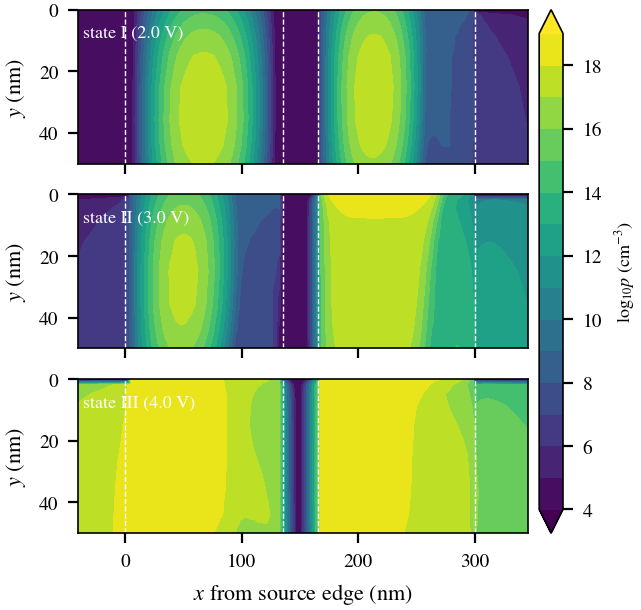
\includegraphics[width=\columnwidth]{figL_hole_maps.png}
\caption{세 상태의 정공 밀도 $\log_{10}p$ (기준 소자 up sweep; 점선: source 끝 0~nm, island 135--165~nm, drain 끝 300~nm). 상태 I: 두 body 모두 꺼짐. 상태 II: 오른쪽 body만 정공으로 채워짐. 상태 III: 두 body 모두 채워지고 island만 비어 있다. 데이터: \dpath{1007\_ddsplit/DDS\_BASE\_SNAP\_T\_tr\_N} (\texttt{.str}, 스냅샷 번호: \dpath{1007\_ddsplit/mech\_DDS\_BASE\_SNAP.dat}). 코드: \dpath{paper/make\_figs\_ext.py}, \dpath{1007\_ddsplit/mech2\_ddsplit.py}.}
\label{fig:holes}
\end{figure}

\textbf{꺼짐과 Si lifetime.} 기준 소자는 두 번째 래치가 완만하게 꺼지는 것처럼 보였다. 스냅샷을 보면 실제 꺼짐은 2.3$\rightarrow$2.2~V 사이에서 급격하다(장벽 0.27$\rightarrow$0.60~eV). 그 앞의 3.0$\rightarrow$2.3~V는 \textbf{켜진 채 전류가 줄어드는} 구간이다. 켜진 상태는 $I_{ii}$가 재결합을 이기고 남은 정공으로 body를 순방향으로 유지하는 동안 지속된다. $\tau_{Si}=10^{-7}$~s에서는 마지막 켜진 점(2.3~V, $I_e=10^{-7}$~A)에서도 생성 정공의 29\%만 재결합하여 여유가 크다. 그래서 작은 전류까지 버틴다. $\tau_{Si}=10^{-8}$~s에서는 2.76~V에서 이미 78\%를 잃는다. 그래서 \textbf{큰 holding current}($5.5\times10^{-7}$~A)에서 2.76$\rightarrow$2.74~V 사이에 6자리가 한 번에 떨어진다 [Fig.~\ref{fig:off}]. 즉 Si \textit{lifetime}은 \textit{holding current}를 올려 꺼짐을 급격하게 만드는 손잡이이다. 대가로 켜는 데에도 정공이 더 필요해 두 래치 전압이 함께 오른다 ($10^{-8}$~s: 2.95/3.94~V).

\begin{figure}[!t]
\centering
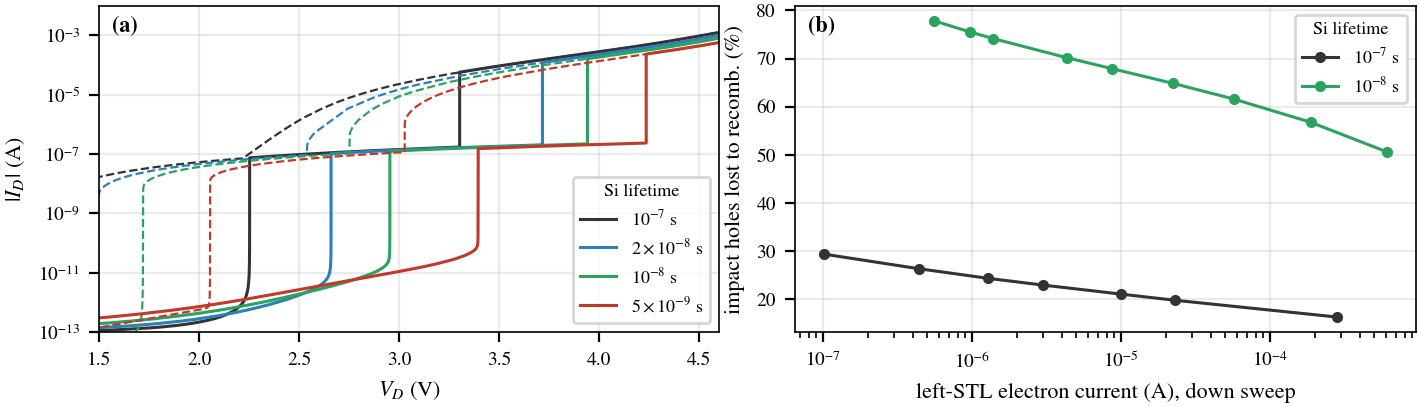
\includegraphics[width=\columnwidth]{fig7_turnoff.png}
\caption{Si \textit{lifetime}과 급격한 꺼짐. (a) $\tau_{Si}$에 따른 $|I_D|$--$V_D$: 수명이 짧을수록 두 번째 래치가 점프로 꺼진다 (OFF 폭 0.26$\rightarrow$0.04~V). (b) Down sweep에서 왼쪽 STL의 \textit{impact} 정공 중 재결합으로 잃는 비율. 데이터: \dpath{1007\_ddsplit/DDS\_\{BASE,TE2em8,TE1em8,TE5em9\}.log\_tr.log}, \dpath{1007\_ddsplit/mech2\_DDS\_\{BASE,TE8\}\_SNAP.dat}.}
\label{fig:off}
\end{figure}

\section{설계 공간 (Design Space)}
기준 소자에서 변수 하나씩 바꾼 DD MixedMode \textit{split} 86개를 계산하였다 [Fig.~\ref{fig:knobs}, Table~\ref{tab:knob}]. 48/50개(1--3차)에서 래치가 두 번이었다. 두 래치는 서로 다른 손잡이로 \textbf{독립적으로} 조절된다. $N_{A,R}$은 첫 번째 래치(1.24--2.51~V), $N_{A,L}$은 두 번째 래치(2.28--4.01~V)를 움직인다. $V_G$는 둘을 함께 움직이고, $R_{tap}$은 래치 전압이 아니라 두 점프의 크기를 나눈다(첫 번째 4.3$\rightarrow$1.9자리, 두 번째 0.7$\rightarrow$3.9자리, $R_{tap}=3\times10^5\rightarrow3\times10^8~\Omega$). 섬 \textit{lifetime}은 $10^{-10}$~s까지는 분리가 유지되고 $10^{-9}$~s에서 두 래치가 합쳐진다. 섬 폭 100~nm에서는 왼쪽 래치가 사라진다.

\begin{figure}[!t]
\centering
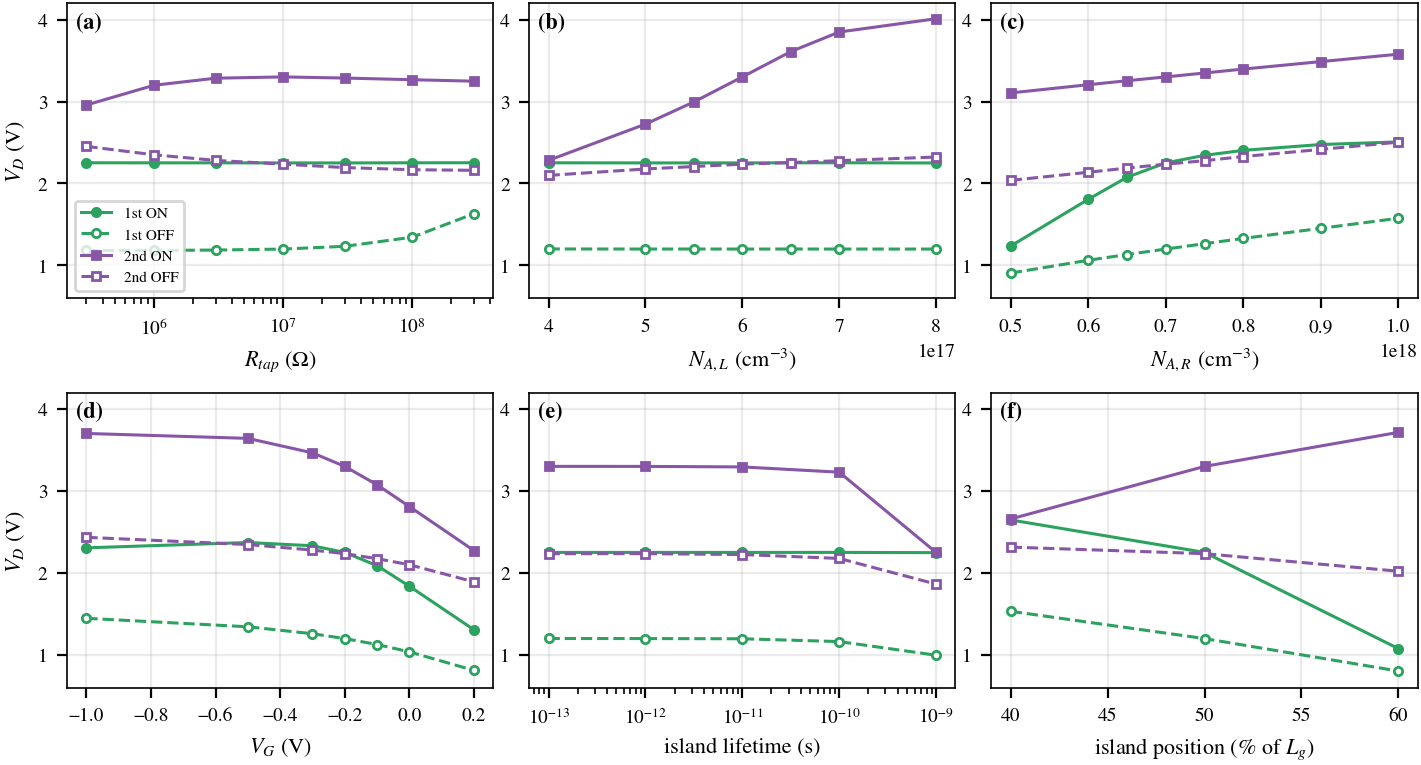
\includegraphics[width=\columnwidth]{fig8_knobs.png}
\caption{설계 손잡이: 두 래치의 ON(실선)/OFF(점선) 전압. (a) $R_{tap}$, (b) 왼쪽 body 도핑, (c) 오른쪽 body 도핑, (d) $V_G$, (e) 섬 \textit{lifetime}, (f) 섬 위치. 데이터: \dpath{1007\_ddsplit/ddsplit\_summary.dat} (원본: \dpath{1007\_ddsplit/DDS\_*.log\_tr.log}, 덱 생성: \dpath{1007\_ddsplit/make\_ddsplit.py}).}
\label{fig:knobs}
\end{figure}

\begin{table}[!t]
\caption{설계 손잡이 요약 (DD split, 데이터: \dpath{1007\_ddsplit/ddsplit\_summary.dat}, \dpath{ddsplit\_rect.dat})}
\label{tab:knob}
\centering\footnotesize
\begin{tabular}{@{}p{0.23\columnwidth}p{0.33\columnwidth}p{0.34\columnwidth}@{}}
\toprule
손잡이 & 올리면 & 대가 \\ \midrule
$N_{A,R}$ & 1번째 래치 상승, 루프 1 넓어짐 & 두 루프 간격 감소 \\
$N_{A,L}$ & 2번째 래치 상승 & $5\times10^{17}$ 이하에서 래치 소멸 \\
$V_G$ ($\uparrow$) & 두 래치 함께 하강 & 루프 1 좁아짐 \\
$R_{tap}$ & 2번째 점프 커짐 & 1번째 점프 작아짐 \\
$\tau_{Si}$ ($\downarrow$) & 급격한 꺼짐 & 두 래치 상승 \\
섬 위치 (drain 쪽) & 루프 분리 & 65\% 이상에서 1번째 래치 소멸 \\
drain 직렬 R & 평평한 윗변 & 2번째 꺼짐 완만 \\ \bottomrule
\end{tabular}
\end{table}

\subsection{변수별 Id-Vd (1--3차 split, $\tau_{Si}=10^{-7}$~s)}
Fig.~\ref{fig:ddsplit}은 변수 하나씩 바꾼 split의 Id-Vd를 변수별로 겹친 것이다 (굵은 선: 기준 소자). 수치는 부록 Table~\ref{tab:all}에 있다.

\textbf{$R_{tap}$} [Fig.~\ref{fig:ddsplit}(a)]. 300~k$\Omega$--300~M$\Omega$에서 첫 번째 래치는 2.25~V로 고정이고, 두 번째 래치는 2.96--3.30~V로 약간만 움직인다. 바뀌는 것은 \textbf{상태 II의 전류 수준}이다. $R_{tap}$이 클수록 같은 섬 전위에 필요한 전류가 작아 상태 II가 낮아지고(300~k$\Omega$: $\sim10^{-6}$~A, 300~M$\Omega$: $\sim10^{-8}$~A), 첫 번째 점프는 작아지고 두 번째 점프는 커진다. 오른쪽 꺼짐 전압은 1.18~V(300~k)에서 1.63~V(300~M)로 오른다.

\textbf{$N_{A,L}$} [Fig.~\ref{fig:ddsplit}(b)]. 첫 번째 래치는 2.25~V로 그대로이고 두 번째 래치만 2.28(4e17), 2.72(5e17), 3.00(5.5e17), 3.30(6e17), 3.61(6.5e17), 3.85(7e17), 4.01~V(8e17)로 오른다. $4\times10^{17}$에서는 두 래치가 30~mV로 붙어 거의 한 번처럼 보인다. 왼쪽 도핑은 두 번째 래치 전압의 독립 손잡이이다.

\textbf{$N_{A,R}$} [Fig.~\ref{fig:ddsplit}(c)]. 첫 번째 래치가 1.24(5e17)에서 2.51~V(1e18)로 오른다. 두 번째 래치도 3.10--3.58~V로 따라 오르지만 변화폭은 첫 번째의 약 40\%이다. 오른쪽 꺼짐 전압도 0.91에서 1.58~V로 올라, 첫 번째 루프가 통째로 이동한다.

\textbf{$V_G$} [Fig.~\ref{fig:ddsplit}(d)]. $V_G$를 $-1.0$에서 $+0.2$~V로 올리면 두 래치가 함께 내려간다(첫 번째 2.31$\rightarrow$1.31~V, 두 번째 3.70$\rightarrow$2.27~V). $V_G\ge0$에서는 채널이 약하게 열려 상태 I의 누설이 늘고 첫 번째 래치가 완만해진다. $V_G\le-0.5$~V에서는 첫 번째 래치가 2.3--2.4~V에서 더 오르지 않는다.

\textbf{섬 \textit{lifetime}} [Fig.~\ref{fig:ddsplit}(e)]. $\tau_{0,isl}=10^{-13}$--$10^{-10}$~s(실효 $5\times10^{-17}$--$5\times10^{-14}$~s)에서는 결과가 거의 같다(두 번째 래치 3.23--3.30~V). $\tau_{0,isl}=10^{-9}$~s(실효 $5\times10^{-13}$~s)에서는 두 래치가 2.248/2.250~V로 \textbf{합쳐진다}. Island 정공 확산 계수를 $D_p\approx1.3$~cm$^2$/s로 두면 확산 길이 $L_p=\sqrt{D_p\tau_{eff}}$는 각각 약 2.5~nm와 8~nm이고, 30~nm island를 건너는 정공 비율 $\sim e^{-W_{IS}/L_p}$는 $10^{-5}$에서 $10^{-2}$ 수준으로 커진다(추정). 이 정도면 가로 PNP 결합이 되살아난다. 따라서 분리에 필요한 island 실효 \textit{lifetime}은 약 $5\times10^{-14}$~s 이하, 즉 $L_p\ll W_{IS}$이다. 섬 \textit{lifetime} 기본값($\tau_0=10^{-7}$~s, 실효 $5\times10^{-11}$~s)에서 결합이 일어난 Section~III의 결과와도 일치한다.

\textbf{섬 폭과 위치} [Fig.~\ref{fig:ddsplit}(f),(g)]. 섬 폭을 20$\rightarrow$50~nm로 넓히면 두 body가 짧아져 두 래치가 2.36/3.53에서 1.92/2.79~V로 내려간다. 100~nm에서는 왼쪽 래치가 사라지고 오른쪽은 0.88~V에서 완만하게 켜진다. 섬을 source 쪽(40\%)으로 옮기면 오른쪽 body가 길어져 첫 번째 래치가 2.65~V로 오르고 두 번째(2.66~V)와 합쳐진다. Drain 쪽(60\%)으로 옮기면 1.08/3.72~V로 \textbf{두 래치 간격이 2.6~V}까지 벌어진다.

\textbf{$T_{si}$와 ramp 속도} [Fig.~\ref{fig:ddsplit}(h),(i)]. $T_{si}=30$~nm는 1.82/2.70~V, 70~nm는 2.35/3.53~V로 두 래치를 함께 움직인다. Ramp 속도를 0.07--7~V/ms로 100배 바꾸면 첫 번째 래치가 0.1--0.2~V, 두 번째는 0.06~V 이내로 이동한다. 7~V/ms에서는 상태 I에 변위전류($\sim10^{-12}$~A)가 보인다. 0.7~V/ms는 준정적에 가깝다.

\begin{figure*}[!t]
\centering
\includegraphics[width=\textwidth]{figI_dd_splits.pdf}
\caption{DD MixedMode split: 변수별 $|I_D|$--$V_D$ (실선 up, 점선 down, 굵은 선: 기준 소자). (a) $R_{tap}$ ($\Omega$), (b) 왼쪽 body 도핑, (c) 오른쪽 body 도핑, (d) $V_G$ (V), (e) 섬 \textit{lifetime} (s), (f) 섬 폭, (g) 섬 중심 위치 ($L_g$ 대비), (h) Si 두께, (i) drain ramp 속도. 데이터: \dpath{1007\_ddsplit/DDS\_\{BASE,R*,NL*,NR*,VG*,TAU*,WISL*,XS40,XS60,TSI*,RATE*\}.log\_tr.log}, 덱: \dpath{1007\_ddsplit/DDS\_*.in} (생성: \dpath{1007\_ddsplit/make\_ddsplit.py}). 코드: \dpath{paper/make\_figs\_ext.py}.}
\label{fig:ddsplit}
\end{figure*}

\subsection{Si \textit{lifetime} $10^{-8}$~s 위에서의 재조정 (4차 split)}
$\tau_{Si}$를 줄이면 꺼짐이 급격해지지만 두 래치가 함께 오른다 [Fig.~\ref{fig:te8}(a)]. $\tau_{Si}=5\times10^{-9}$, $10^{-8}$, $2\times10^{-8}$, $5\times10^{-8}$, $10^{-7}$~s에서 래치는 3.39/4.23, 2.95/3.94, 2.66/3.72, 2.40/3.48, 2.25/3.30~V, 두 번째 꺼짐 폭($|I_S|$ $10^{-6}\rightarrow10^{-8}$~A 구간)은 0.000, 0.044, 0.20, 0.30, 0.26~V이다. $10^{-9}$~s에서는 4.63~V의 한 번만 남았다. 그래서 $\tau_{Si}=10^{-8}$~s를 기준으로 다른 변수를 다시 조정하였다.

$N_{A,L}$은 여기서도 두 번째 래치만 움직인다(5e17: 3.32, 5.5e17: 3.62, 6.5e17: 4.24~V) [Fig.~\ref{fig:te8}(b)]. 단, 도핑을 낮추면 꺼짐 폭이 0.10~V로 늘었다. $N_{A,R}$을 $5\times10^{17}$로 낮추면 첫 번째 래치가 1.67~V로 내려가 두 루프가 \textbf{0.86~V 간격으로 처음 분리}되었다 [Fig.~\ref{fig:te8}(c)]. $V_G=0$은 두 래치를 0.4~V 내리고(2.54/3.55~V), $R_{tap}$ 3~M--30~M$\Omega$는 오른쪽 꺼짐 전압만 1.61--1.87~V로 바꾸었다 [Fig.~\ref{fig:te8}(d)]. 섬 60\%는 1.45/4.78~V로 간격 1.12~V, 섬 폭 50~nm는 2.48/3.34~V, 섬 \textit{lifetime} $10^{-11}$~s는 기준과 같았다 [Fig.~\ref{fig:te8}(e)]. 조합 중 $N_{A,R}=N_{A,L}=5\times10^{17}$은 1.67/3.07~V(간격 0.78~V)였고, drain 30~k$\Omega$는 상태 III 전류를 $10^{-4}$~A 아래로 묶었다 [Fig.~\ref{fig:te8}(f)].

\begin{figure*}[!t]
\centering
\includegraphics[width=\textwidth]{figJ_te8.pdf}
\caption{Si \textit{lifetime} $10^{-8}$~s 기준 split (굵은 선: \texttt{DDS\_TE1em8}). (a) Si \textit{lifetime}, (b) 왼쪽 도핑, (c) 오른쪽 도핑, (d) $V_G$와 $R_{tap}$, (e) 섬 위치/폭/\textit{lifetime}, (f) 조합과 drain 직렬 저항 30~k$\Omega$. 데이터: \dpath{1007\_ddsplit/DDS\_\{TE5em9,TE1em8,TE2em8,TE5em8,BASE,RD3e4\_TE1em8\}.log\_tr.log}, \dpath{1007\_ddsplit/DDS\_TE8\_*.log\_tr.log}.}
\label{fig:te8}
\end{figure*}

\subsection{두 사각형 \textit{loop}의 변수별 조정 (5차 split)}
섬 60\%, $\tau_{Si}=10^{-8}$~s(\texttt{TE8\_XS60})를 기준으로 여섯 변수를 바꾸었다 [Fig.~\ref{fig:rectall}].
(a) 섬 위치: 55\%는 2.22/4.44~V(간격 0.46~V), 60\%는 1.45/4.78~V(1.12~V)이다. 65\%와 70\%에서는 오른쪽 body가 너무 짧아 첫 번째 래치가 사라지고 0--1~V에서 연속적으로 켜졌다.
(b) $N_{A,L}$ 5, 5.5, 6$\times10^{17}$: 두 번째 래치 4.08, 4.47, 4.78~V. 첫 번째 루프는 변하지 않는다.
(c) $V_G$ 0, $-0.1$, $-0.2$~V: 1.16/4.37, 1.32/4.62, 1.45/4.78~V로 두 루프가 함께 이동한다.
(d) $N_{A,R}$ 8e17: 1.88/4.88~V, 첫 번째 루프 폭이 0.22에서 0.49~V로 넓어진다. 1e18: 2.74/5.09~V로 간격이 0.10~V로 줄고, 오른쪽 래치가 2~mV 간격의 두 점프로 검출되었다.
(e) $\tau_{Si}$ $5\times10^{-9}$~s: 1.61/5.22~V, 간격 1.25~V, 두 꺼짐 폭 0.001/0.008~V로 가장 급격하다. $2\times10^{-8}$~s: 1.31/4.44~V, 꺼짐 폭 0.16~V. $10^{-7}$~s: 1.08/3.72~V, 꺼짐 폭 0.29~V.
(f) Drain 직렬 저항 100~k, 300~k, 1~M$\Omega$: 상태 III 전류가 각각 $\sim3\times10^{-5}$, $10^{-5}$, $3\times10^{-6}$~A로 평평해지는 대신 두 번째 꺼짐 폭이 0.12, 0.34, 0.95~V로 늘었다. 소자에 걸리는 전압이 $V_D-I_DR_D$이므로, 꺼지는 동안 전류가 줄면 소자 전압이 다시 올라 같은 전이가 인가 전압 축에서 넓게 퍼지기 때문이다.

\begin{figure*}[!t]
\centering
\includegraphics[width=\textwidth]{figK_rect.pdf}
\caption{섬 60\%, $\tau_{Si}=10^{-8}$~s 기준(굵은 선: \texttt{DDS\_TE8\_XS60})의 사각형 \textit{loop} split. (a) 섬 위치, (b) 왼쪽 도핑, (c) $V_G$, (d) 오른쪽 도핑, (e) Si \textit{lifetime}, (f) drain 직렬 저항. 데이터: \dpath{1007\_ddsplit/DDS\_TE8\_XS\{55,60,65,70\}*.log\_tr.log}, \dpath{1007\_ddsplit/DDS\_\{TE5em9,TE2em8\}\_XS60.log\_tr.log}, \dpath{1007\_ddsplit/DDS\_XS60.log\_tr.log}; 루프 지표: \dpath{1007\_ddsplit/ddsplit\_rect.dat}.}
\label{fig:rectall}
\end{figure*}

\subsection{조합 소자}
응용에서는 두 \textit{hysteresis loop}가 겹치지 않고, 모서리가 급격하며, 각 상태의 전류가 평평한 것이 좋다. $\tau_{Si}=10^{-8}$~s만 쓰면 두 루프가 겹친다(루프 2 꺼짐 2.75~V < 루프 1 켜짐 2.95~V). 섬을 $L_g$의 60\%로 옮겨 오른쪽 body를 짧게 하면 루프 1이 1.23--1.45~V로 내려가고, 루프 2(2.56--4.78~V)와 \textbf{1.12~V 간격}으로 분리된다. 두 꺼짐 모두 점프이다(OFF 폭 0.03/0.06~V) [Fig.~\ref{fig:rect}(a)]. 오른쪽 도핑을 $8\times10^{17}$으로 올리면 루프 1이 1.39--1.88~V로 넓어지고 간격은 0.78~V가 된다 [Fig.~\ref{fig:rect}(b)]. Drain 직렬 저항은 상태 III의 전류를 평평하게 하지만(기울기 3.1$\rightarrow$1.5자리, 100~k$\Omega$) 두 번째 꺼짐을 완만하게 한다 [Fig.~\ref{fig:rect}(c)]. 이를 조합한 소자는 Fig.~\ref{fig:rect}(d)와 같다. \PAPERDEVICE

\begin{figure}[!t]
\centering
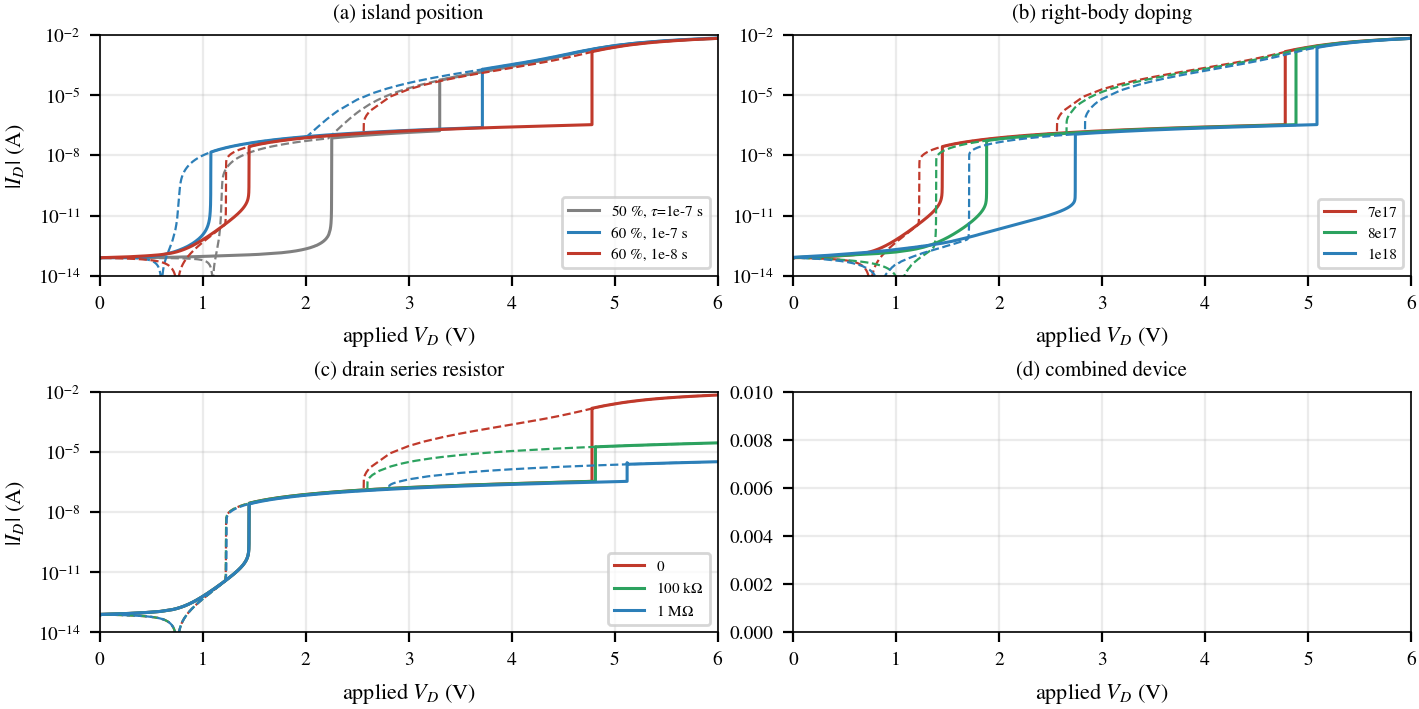
\includegraphics[width=\columnwidth]{fig9_rectangles.png}
\caption{분리된 두 사각형 \textit{loop} (실선 up, 점선 down). (a) 섬 위치와 $\tau_{Si}$, (b) 오른쪽 body 도핑, (c) drain 직렬 저항, (d) 조합 소자(섬 60\%, $N_{A,R}=8\times10^{17}$, drain 100~k$\Omega$, $\tau_{Si}=10^{-8}$/$5\times10^{-9}$~s). 데이터: \dpath{1007\_ddsplit/DDS\_\{BASE,XS60,TE8\_XS60,TE8\_XS60\_NR8e17,TE8\_XS60\_NR1e18,TE8\_XS60\_RD1e5,TE8\_XS60\_RD1e6\}.log\_tr.log}, \dpath{1007\_ddsplit/DDS\_\{TE8,TE5em9\}\_XS60\_NR8e17\_RD1e5.log\_tr.log}.}
\label{fig:rect}
\end{figure}

\section{모델의 한계 (Model Limitations)}
\textbf{DD vs hcte.} DD는 국소 전계로 \textit{impact ionization}을 계산하므로 짧은 채널에서 과대평가한다. 실제로 standalone 왼쪽 STL에서 DD 래치 전압은 hcte보다 0.7--0.8~V 낮았다. 또 4e17, 5e17에서는 $V_D<E_g/q$ 부근의 래치가 나타났다 [Fig.~\ref{fig:left}(b)]. hcte로는 각 STL 단독의 래치와 본 소자의 첫 번째 래치까지 확인하였다. 그러나 전체 소자를 hcte로 계산하면 \textbf{3.6--5.3~V에서 모두 멈추었다} [Fig.~\ref{fig:hcte}]. 증상은 매번 같았다: 오른쪽 drain 접합 표면($x\approx285$~nm)의 전자 온도가 $10^4$~K를 넘고 time step이 $10^{-25}$~s로 붕괴한다. 연립 Newton, 1~nm 격자, 온도 허용치 완화, MixedMode, graded drain, 전자 온도만 계산(\texttt{hcte.el}), $R_{tap}$ 10--100~M$\Omega$를 모두 시도하였다. 그러나 멈추는 위치를 두 번째 래치(약 5.6--7~V)까지 옮기지 못하였다. 오히려 $R_{tap}$이 클수록 일찍 멈추었다. 따라서 두 번째 래치는 DD 결과이며, 절대 전압은 hcte 대비 낮게 추정된 값이다.

\begin{figure}[!t]
\centering
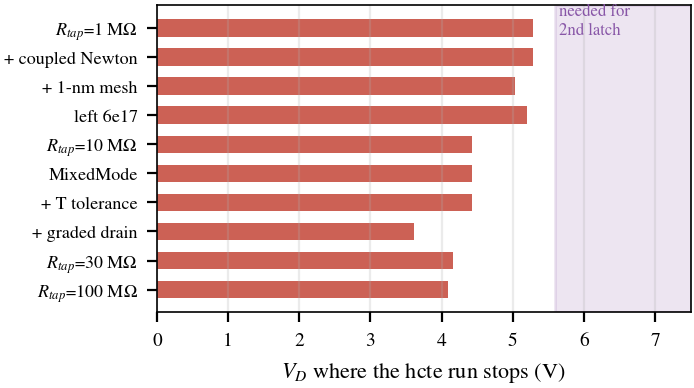
\includegraphics[width=\columnwidth]{fig10_hcte.png}
\caption{hcte 계산이 멈춘 $V_D$ (각 run의 마지막 수렴점). 보라색: 두 번째 래치에 필요한 영역. 데이터: \dpath{1001/tap/TAPT\_ISL\_W30LK\_*\_R*\_VGm0p2.log}, \dpath{1001/tap/MM\_TAPT\_ISL\_W30LK\_*\_HC*.log\_tr.log}; 수렴 실패 기록: README Step~11.}
\label{fig:hcte}
\end{figure}

\begin{table}[!t]
\caption{hcte 전체 소자 계산의 수렴 실패 완화 시도 (덱: \dpath{1001/tap/})}
\label{tab:hcte}
\centering\scriptsize
\begin{tabular}{@{}r@{\;}p{0.5\columnwidth}@{\;}p{0.36\columnwidth}@{}}
\toprule
\# & 시도 & 멈춘 $V_D$ / 결과 \\ \midrule
0 & 기준: $R_{tap}$ 1~M$\Omega$, 왼쪽 3e17 & 5.284~V (가짜 점프) \\
1 & 연립 Newton (5.0~V에서 재시작) & 5자리 일치, 5.284~V \\
2 & \texttt{dt.max} $2\times10^{-8}$~s & 효과 없음 \\
3 & 4.5~V에서 DD로 재시작 & 모델 불연속 (폐기) \\
4 & drain 접합 격자 5$\rightarrow$1~nm & 5.033~V \\
5 & 왼쪽 6e17 & 5.201~V \\
6 & $R_{tap}$ 10~M$\Omega$ & 4.422~V \\
7 & MixedMode & 4자리 일치, 20배 빠름, 4.422~V \\
8 & Gaussian drain 경사 (10~nm) & 3.607~V \\
9 & 전자 온도만 (\texttt{hcte.el}) & $V_D=0$에서 발산 \\
10 & 온도 허용치 100배 완화 & 4.422~V \\
11 & $R_{tap}$ 30~M$\Omega$ & 4.167~V \\
12 & $R_{tap}$ 100~M$\Omega$ & 4.084~V \\ \bottomrule
\end{tabular}
\end{table}

hcte 실패를 완화하려는 12가지 시도를 Table~\ref{tab:hcte}에 정리하였다. 수치 설정(solver, time step, 격자, 허용치)으로는 멈추는 위치가 거의 바뀌지 않았다. 구조 변경 중 $R_{tap}$을 키우면 오히려 일찍 멈추었다(1~M: 5.0--5.3, 10~M: 4.42, 30~M: 4.17, 100~M: 4.08~V). 섬 전위를 올리려면 $R_{tap}$이 커야 하므로 hcte가 버티는 방향과 반대이다. Fig.~\ref{fig:hcdiag}(a)는 멈추기 직전의 전자 온도 단면이다. Drain 접합 바로 앞($x\approx285$~nm)에서 12,000~K에 이르고 접합을 지나 격자 두 칸 안에 300~K로 떨어진다. 이 급경사가 격자 세분화의 동기였지만 1~nm 격자에서도 해결되지 않았다. 따라서 수치 기법 문제라기보다 이 소자에서 hcte 해 자체가 불안정해지는 것으로 본다.

\begin{figure}[!t]
\centering
\includegraphics[width=\columnwidth]{figM_hcte_diag.pdf}
\caption{hcte 실패 진단. (a) 5.25~V 전자 온도 $T_n$ 단면 (표면, 중간 깊이; 점선: drain 경계). (b) $R_{tap}=1$~M$\Omega$ run의 마지막 45점: time step이 $10^{-25}$~s로 붕괴한 뒤 $|I_G|$가 $10^{-13}$에서 $10^{-3}$~A로 뛰는 가짜 점프. 데이터: \dpath{1001/tap/TAPT\_ISL\_W30LK\_L3\_R7\_R1e6\_RS50\_NEWT\_VGm0p2\_UP\_5p25.str}, \dpath{1001/tap/TAPT\_ISL\_W30LK\_L3\_R7\_R1e6\_UD7S\_VGm0p2.log}.}
\label{fig:hcdiag}
\end{figure}

\textbf{수치 오류 판정.} 초기 hcte run(1~M$\Omega$)에서는 5.28~V에서 $I_D$, $I_S$가 음수로 튀어 두 번째 래치처럼 보였다. 그러나 이 점프 동안 time step은 $10^{-25}$~s로 붕괴하고, 내부 전위는 소수점 셋째 자리까지 고정되어 있었다. 또 gate 변위전류가 $10^{-2}$~A, KCL 잔차가 $10^{-2}$~A였다. 본 연구는 이 네 가지 기준으로 모든 래치를 검증하였다.

\textbf{면적: STL 두 개를 직렬로 쓰는 것과의 비교.} 같은 등가 회로(Fig.~\ref{fig:circuit})를 개별 소자로 만드는 경우와 채널 방향 길이를 비교하였다 (Table~\ref{tab:area}). Scalable CMOS 설계 규칙(gate 길이 $2\lambda$, contact $2\lambda$, contact--gate 간격 $2\lambda$, contact의 active 여유 $1.5\lambda$, active 간격 $3\lambda$)을 쓰고, 각 STL의 body를 최소 gate 길이 $2\lambda$로 두었다. 개별 STL 두 개를 금속으로 잇는 경우는 $29\lambda$, 가운데 확산을 공유하되 그 노드에 contact를 다는 적층(stacked) 구조는 $21\lambda$이다. 제안 소자는 gate 하나가 두 body와 island를 덮고, island 노드를 위쪽 contact 대신 BOX 관통 via로 꺼내므로 $15\lambda+W_{IS}$이다 ($W_{IS}=30$~nm는 $\lambda=67.5$~nm에서 $0.44\lambda$). 즉 적층 구조보다 약 27\%, 개별 소자보다 약 47\% 짧다. $R_{tap}$은 세 경우 모두 필요하므로 비교에서 뺐다. 이 이득은 island 노드를 위쪽 contact 없이 아래로 꺼낼 수 있다는 가정에 달려 있으며, 그 대가로 BOX 관통 via와 그 아래 배선(예: ground-plane 또는 후면 배선)이 필요하다. 단자 수는 S, D, G, tap의 4개로, 적층 구조(S, D, G$_1$, G$_2$, 중간 노드)보다 적다.

\begin{table}[!t]
\caption{채널 방향 길이 비교 (scalable 설계 규칙, 단위 $\lambda$; $R_{tap}$ 제외)}
\label{tab:area}
\centering\scriptsize
\begin{tabular}{@{}p{0.34\columnwidth}p{0.36\columnwidth}c@{}}
\toprule
구성 & 길이 내역 & 합계 \\ \midrule
개별 STL 2개 + 금속 연결 & $2\times(1.5+2+2+2+2+2+1.5)+3$ & $29\lambda$ \\
적층, 중간 노드 contact & $5.5+2+6+2+5.5$ & $21\lambda$ \\
\textbf{제안 소자} (gate 1개, island via) & $5.5+(2+W_{IS}+2)+5.5$ & $\mathbf{15\lambda}+W_{IS}$ \\ \bottomrule
\end{tabular}
\end{table}

\textbf{공정 구현.} 분리 조건은 island 실효 \textit{lifetime} $\le5\times10^{-14}$~s, 즉 정공 확산 길이가 island 폭보다 훨씬 짧은 것이다. 이온 주입 손상으로 얻을 수 있는 Si \textit{lifetime}은 ps 수준이므로 이 값을 손상만으로 만들기는 어렵다. 같은 역할을 하는 현실적인 구조는 \textbf{정공을 무한히 빨리 소멸시키는 금속성 sink}이다. 예를 들어 Si 두께 전체를 관통하는 silicide island(또는 금속 via)를 섬 자리에 두고 BOX 아래 tap으로 연결하면 된다. 이때 Section~III의 top contact(C)처럼 contact가 얕으면 정공이 그 아래로 지나가므로 \textbf{Si 전체 두께를 관통}해야 한다. 이 구조(금속 코어 10~nm + n$^+$ shell, island lifetime은 줄이지 않음)를 TCAD로 확인하는 계산을 진행 중이다 (덱: \dpath{1010\_sink/SINK\_*.in}). Body의 $\tau_{0,Si}=10^{-8}$~s(실효 0.7~ns)는 Au/Pt 확산이나 전자선/양성자 조사 같은 기존 \textit{lifetime control} 기술의 범위이며(floating-body 메모리의 lifetime engineering 예~\cite{kim_lifetime}), $R_{tap}$(1--10~M$\Omega$)은 고저항 poly-Si 저항으로 집적할 수 있다.

\section{결론 (Conclusion)}
두 개의 직렬 STL을 한 SOI 소자로 구현하여 \textbf{두 번의 래치}를 얻었다. 이를 위해 세 가지가 필요했다: (1) n$^+$ island로 body를 물리적으로 나누기, (2) island를 $R_{tap}$으로 접지하여 직렬 제약을 풀기, (3) island \textit{lifetime}을 줄여 가로 PNP 결합을 끊기. 여기에 왼쪽 body를 래치 가능한 도핑($6\times10^{17}$)으로 정하였다. \texttt{.str} 기반 \textit{hole balance}로 각 래치가 해당 STL의 \textit{impact ionization} 정공이 재결합을 이겨 장벽이 무너지는 순간임을 보였다. 꺼짐의 급격함은 Si \textit{lifetime}이 정하는 \textit{holding current}로 설명하였다. 두 래치는 $N_{A,R}$, $N_{A,L}$, $V_G$, $R_{tap}$으로 독립 조절되며, 섬 위치 60\%와 $\tau_{Si}=10^{-8}$~s에서 두 \textit{hysteresis loop}가 1.1~V 간격으로 분리된다. 남은 과제는 에너지 균형 모델에서의 두 번째 래치 확인과 \textit{lifetime engineering}의 공정 구현이다.

\appendix[전체 DD split 결과]
Table~\ref{tab:all}은 계산한 모든 DD MixedMode split의 래치 지표이다. 이름은 기준 소자(\texttt{BASE}: Table~\ref{tab:param})에서 바꾼 변수이다: R($R_{tap}$), NL/NR(왼/오른쪽 도핑), VG, TAU(섬 \textit{lifetime}), TE(Si \textit{lifetime}; TE8 $=10^{-8}$~s), WISL(섬 폭 nm), XS(섬 위치 \%), TSI, RATE(V/ms), RD(drain 직렬 $\Omega$), SNAP(\texttt{.str} 스냅샷 저장 run).

\begin{table*}[!t]
\caption{전체 DD split 결과. $n$: up sweep 래치 수, $V_{on,R/L}$: 오른쪽/왼쪽 래치 전압, $V_{off,R}$: $I_{tap}<10^{-9}$~A, $V_{off,L}$: $|I_S|<10^{-8}$~A, $\Delta V_{off}$: 왼쪽 꺼짐 폭($|I_S|$ $10^{-6}\rightarrow10^{-8}$~A), sep: $V_{off,L}-V_{on,R}$ (양수면 두 루프 분리). 단위 V. 데이터: \dpath{1007\_ddsplit/ddsplit\_summary.dat}, \dpath{1007\_ddsplit/ddsplit\_rect.dat} (코드: \dpath{1007\_ddsplit/analyze\_ddsplit.py}).}
\label{tab:all}
\centering\scriptsize
\begin{tabular}{@{}l@{\,}c@{\,}c@{\,}c@{\,}c@{\,}c@{\,}c@{\,}c@{}}\toprule
split & $n$ & $V_{on,R}$ & $V_{on,L}$ & $V_{off,R}$ & $V_{off,L}$ & $\Delta V_{off}$ & sep \\ \midrule
BASE & 2 & 2.25 & 3.30 & 1.20 & 2.24 & 0.26 & -0.01 \\
BASE\_SNAP & 2 & 2.25 & 3.30 & 1.20 & 2.23 & 0.24 & -0.02 \\
NL4e17 & 2 & 2.25 & 2.28 & 1.20 & 2.10 & 0.33 & -0.15 \\
NL5e17 & 2 & 2.25 & 2.72 & 1.20 & 2.18 & 0.32 & -0.07 \\
NL5p5e17 & 2 & 2.25 & 3.00 & 1.20 & 2.21 & 0.29 & -0.04 \\
NL5p5e17\_R3e6 & 2 & 2.25 & 2.97 & 1.19 & 2.26 & 0.23 & 0.01 \\
NL5p5e17\_R3e7 & 2 & 2.25 & 2.99 & 1.23 & 2.17 & 0.33 & -0.08 \\
NL6p5e17 & 2 & 2.25 & 3.61 & 1.20 & 2.26 & 0.24 & 0.00 \\
NL6p5e17\_R3e6 & 2 & 2.25 & 3.60 & 1.19 & 2.30 & 0.20 & 0.05 \\
NL6p5e17\_R3e7 & 2 & 2.25 & 3.59 & 1.23 & 2.22 & 0.28 & -0.03 \\
NL7e17 & 2 & 2.25 & 3.85 & 1.20 & 2.28 & 0.22 & 0.03 \\
NL8e17 & 2 & 2.25 & 4.01 & 1.20 & 2.32 & 0.30 & 0.07 \\
NR1e18 & 2 & 2.51 & 3.58 & 1.58 & 2.50 & 0.23 & -0.00 \\
NR5e17 & 2 & 1.24 & 3.10 & 0.91 & 2.04 & 0.33 & 0.80 \\
NR6e17 & 2 & 1.81 & 3.20 & 1.06 & 2.14 & 0.26 & 0.33 \\
NR6p5e17 & 2 & 2.08 & 3.25 & 1.13 & 2.19 & 0.27 & 0.11 \\
NR7p5e17 & 2 & 2.34 & 3.35 & 1.27 & 2.28 & 0.27 & -0.07 \\
NR8e17 & 2 & 2.40 & 3.40 & 1.33 & 2.33 & 0.26 & -0.07 \\
NR9e17 & 2 & 2.48 & 3.49 & 1.45 & 2.42 & 0.30 & -0.06 \\
R1e6 & 2 & 2.25 & 3.20 & 1.18 & 2.35 & 0.22 & 0.10 \\
R1e8 & 2 & 2.25 & 3.27 & 1.34 & 2.17 & 0.31 & -0.09 \\
R3e5 & 2 & 2.25 & 2.96 & 1.18 & 2.45 & 0.15 & 0.20 \\
R3e6 & 2 & 2.25 & 3.28 & 1.19 & 2.28 & 0.22 & 0.03 \\
R3e7 & 2 & 2.25 & 3.29 & 1.23 & 2.19 & 0.31 & -0.06 \\
R3e8 & 2 & 2.25 & 3.25 & 1.63 & 2.16 & 0.34 & -0.09 \\
RATE0p07 & 2 & 2.15 & 3.23 & 1.20 & 2.23 & 0.27 & 0.08 \\
RATE7 & 2 & 2.05 & 3.24 & 1.19 & 2.23 & 0.27 & 0.18 \\
RD1e4 & 2 & 2.25 & 3.30 & 1.20 & 2.23 & 0.27 & -0.02 \\
RD1e5 & 2 & 2.25 & 3.32 & 1.20 & 2.24 & 0.37 & -0.01 \\
RD3e4 & 2 & 2.25 & 3.30 & 1.20 & 2.23 & 0.36 & -0.02 \\
RD3e4\_TE1em8 & 2 & 2.95 & 3.95 & 1.72 & 2.76 & 0.09 & -0.19 \\
TAU1em10 & 2 & 2.25 & 3.23 & 1.16 & 2.18 & 0.26 & -0.07 \\
TAU1em11 & 2 & 2.25 & 3.29 & 1.20 & 2.23 & 0.24 & -0.03 \\
TAU1em13 & 2 & 2.25 & 3.30 & 1.20 & 2.23 & 0.24 & -0.02 \\
TAU1em9 & 2 & 2.25 & 2.25 & 1.00 & 1.86 & 0.32 & -0.38 \\
TE1em8 & 2 & 2.95 & 3.94 & 1.72 & 2.75 & 0.04 & -0.20 \\
TE1em9 & 1 & 4.63 & -- & 4.30 & -- & -- & -- \\
TE2em8 & 2 & 2.66 & 3.72 & 1.50 & 2.54 & 0.20 & -0.12 \\
TE2em8\_XS60 & 2 & 1.31 & 4.44 & 1.05 & 2.34 & 0.16 & 1.03 \\
TE5em8 & 2 & 2.40 & 3.48 & 1.30 & 2.34 & 0.30 & -0.06 \\
TE5em9 & 2 & 3.39 & 4.23 & 2.05 & 3.03 & 0.00 & -0.36 \\
TE5em9\_XS60 & 2 & 1.61 & 5.22 & 1.47 & 2.86 & 0.00 & 1.25 \\
TE8\_NL5e17 & 2 & 2.95 & 3.32 & 1.72 & 2.68 & 0.10 & -0.27 \\
\bottomrule\end{tabular}\hfill
\begin{tabular}{@{}l@{\,}c@{\,}c@{\,}c@{\,}c@{\,}c@{\,}c@{\,}c@{}}\toprule
split & $n$ & $V_{on,R}$ & $V_{on,L}$ & $V_{off,R}$ & $V_{off,L}$ & $\Delta V_{off}$ & sep \\ \midrule
TE8\_NL5p5e17 & 2 & 2.95 & 3.62 & 1.72 & 2.72 & 0.10 & -0.23 \\
TE8\_NL6p5e17 & 2 & 2.95 & 4.24 & 1.72 & 2.78 & 0.03 & -0.17 \\
TE8\_NR5e17 & 2 & 1.67 & 3.69 & 1.33 & 2.53 & 0.06 & 0.86 \\
TE8\_NR5e17\_NL5e17 & 2 & 1.67 & 3.07 & 1.33 & 2.45 & 0.08 & 0.78 \\
TE8\_NR6e17 & 2 & 2.38 & 3.82 & 1.54 & 2.64 & 0.20 & 0.26 \\
TE8\_NR6e17\_NL5p5e17 & 2 & 2.38 & 3.50 & 1.54 & 2.61 & 0.09 & 0.22 \\
TE8\_R3e6 & 2 & 2.95 & 3.95 & 1.61 & 2.77 & 0.05 & -0.19 \\
TE8\_R3e7 & 2 & 2.95 & 3.96 & 1.87 & 2.75 & 0.03 & -0.20 \\
TE8\_SNAP & 2 & 2.95 & 3.94 & 1.72 & 2.75 & 0.05 & -0.20 \\
TE8\_TAU1em11 & 2 & 2.95 & 3.93 & 1.72 & 2.75 & 0.05 & -0.21 \\
TE8\_VG0 & 2 & 2.54 & 3.55 & 1.59 & 2.65 & 0.04 & 0.11 \\
TE8\_VG0\_NL5p5e17 & 2 & 2.54 & 3.22 & 1.59 & 2.60 & 0.06 & 0.07 \\
TE8\_VGm0p1 & 2 & 2.77 & 3.78 & 1.66 & 2.71 & 0.05 & -0.07 \\
TE8\_WISL50 & 2 & 2.48 & 3.34 & 1.57 & 2.52 & 0.08 & 0.04 \\
TE8\_XS55 & 2 & 2.22 & 4.44 & 1.49 & 2.68 & 0.07 & 0.46 \\
TE8\_XS60 & 2 & 1.45 & 4.78 & 1.23 & 2.56 & 0.06 & 1.12 \\
TE8\_XS60\_NL5e17 & 2 & 1.45 & 4.08 & 1.23 & 2.50 & 0.09 & 1.05 \\
TE8\_XS60\_NL5p5e17 & 2 & 1.45 & 4.47 & 1.23 & 2.53 & 0.20 & 1.08 \\
TE8\_XS60\_NL5p5e17\_RD3e5 & 2 & 1.45 & 4.56 & 1.23 & 2.61 & 0.31 & 1.17 \\
TE8\_XS60\_NR1e18 & 3 & 2.74 & 5.09 & 1.71 & 2.84 & 0.02 & 0.10 \\
TE8\_XS60\_NR8e17 & 2 & 1.88 & 4.88 & 1.39 & 2.66 & 0.08 & 0.78 \\
TE8\_XS60\_RD1e5 & 2 & 1.45 & 4.81 & 1.23 & 2.60 & 0.12 & 1.15 \\
TE8\_XS60\_RD1e6 & 2 & 1.45 & 5.12 & 1.23 & 2.81 & 0.94 & 1.36 \\
TE8\_XS60\_RD3e5 & 2 & 1.45 & 4.88 & 1.23 & 2.66 & 0.34 & 1.21 \\
TE8\_XS60\_SNAP & 2 & 1.45 & 4.78 & 1.23 & 2.56 & 0.04 & 1.12 \\
TE8\_XS60\_VG0 & 2 & 1.16 & 4.37 & 1.09 & 2.47 & 0.09 & 1.31 \\
TE8\_XS60\_VGm0p1 & 2 & 1.32 & 4.62 & 1.17 & 2.52 & 0.07 & 1.21 \\
TE8\_XS65 & 1 & -- & 4.93 & 0.88 & 2.43 & 0.07 & -- \\
TE8\_XS65\_NL5e17\_RD3e5 & 1 & -- & 4.46 & 0.88 & 2.44 & 0.33 & -- \\
TE8\_XS70 & 1 & -- & 4.92 & 0.40 & 2.26 & 0.05 & -- \\
TSI30 & 2 & 1.82 & 2.70 & 1.07 & 2.28 & 0.33 & 0.46 \\
TSI70 & 2 & 2.35 & 3.53 & 1.27 & 2.17 & 0.20 & -0.17 \\
VG0 & 2 & 1.84 & 2.81 & 1.04 & 2.10 & 0.34 & 0.26 \\
VGm0p1 & 2 & 2.09 & 3.08 & 1.13 & 2.17 & 0.27 & 0.09 \\
VGm0p3 & 2 & 2.33 & 3.47 & 1.26 & 2.28 & 0.27 & -0.05 \\
VGm0p5 & 2 & 2.37 & 3.64 & 1.34 & 2.35 & 0.29 & -0.03 \\
VGm1p0 & 2 & 2.31 & 3.70 & 1.45 & 2.43 & 0.28 & 0.13 \\
VGp0p2 & 2 & 1.31 & 2.27 & 0.81 & 1.89 & 0.48 & 0.58 \\
WISL100 & 1 & 0.88 & -- & 0.73 & 1.44 & 0.34 & 0.56 \\
WISL20 & 2 & 2.36 & 3.53 & 1.26 & 2.33 & 0.25 & -0.03 \\
WISL50 & 2 & 1.92 & 2.79 & 1.08 & 2.03 & 0.28 & 0.11 \\
XS40 & 2 & 2.65 & 2.66 & 1.53 & 2.32 & 0.28 & -0.33 \\
XS60 & 2 & 1.08 & 3.71 & 0.80 & 2.02 & 0.29 & 0.94 \\
\bottomrule\end{tabular}

\end{table*}

\section*{Data Availability}
모든 덱(\texttt{.in}), 분석 코드, 핵심 log와 그림은 저장소에 있다. Raw \texttt{.str}/\texttt{.out}은 연구 서버의 같은 경로에 있다. 전체 연구 흐름(실패 포함)은 저장소 \texttt{README.md}에 기록하였다.

\begin{thebibliography}{99}
\bibitem{chen_stl} C.-D. Chen, M. Matloubian, R. Sundaresan, B.-Y. Mao, C. C. Wei, and G. P. Pollack, ``Single-transistor latch in SOI MOSFETs,'' \emph{IEEE Electron Device Lett.}, vol.~9, no.~12, pp.~636--638, Dec. 1988.
\bibitem{han_biristor} J.-W. Han and Y.-K. Choi, ``Biristor---Bistable resistor based on a silicon nanowire,'' \emph{IEEE Electron Device Lett.}, vol.~31, no.~8, pp.~797--799, Aug. 2010.
\bibitem{kim_1tdram} D.-O. Kim, D.-I. Moon, and Y.-K. Choi, ``Optimization of bias schemes for long-term endurable 1T-DRAM through the use of the biristor mode operation,'' \emph{IEEE Electron Device Lett.}, vol.~35, no.~2, pp.~220--222, Feb. 2014.
\bibitem{moon_fin} D.-I. Moon, S.-J. Choi, J.-W. Han, S. Kim, and Y.-K. Choi, ``Fin-width dependence of BJT-based 1T-DRAM implemented on FinFET,'' \emph{IEEE Electron Device Lett.}, vol.~31, no.~9, pp.~909--911, Sep. 2010.
\bibitem{han_lif} J.-W. Han and M. Meyyappan, ``Leaky integrate-and-fire biristor neuron,'' \emph{IEEE Electron Device Lett.}, vol.~39, no.~9, pp.~1457--1460, Sep. 2018.
\bibitem{han_mimic} J.-K. Han \emph{et al.}, ``Mimicry of excitatory and inhibitory artificial neuron with leaky integrate-and-fire function by a single MOSFET,'' \emph{IEEE Electron Device Lett.}, vol.~41, no.~2, pp.~208--211, Feb. 2020.
\bibitem{han_sciadv} J.-K. Han \emph{et al.}, ``Cointegration of single-transistor neurons and synapses by nanoscale CMOS fabrication for highly scalable neuromorphic hardware,'' \emph{Sci. Adv.}, vol.~7, no.~32, Art. no. eabg8836, Aug. 2021.
\bibitem{kim_osc} H.-Y. Kim, S.-I. Kim, J.-K. Han, J.-W. Jung, and Y.-K. Choi, ``A single MOSFET-based oscillator on a bulk-silicon wafer,'' \emph{IEEE Electron Device Lett.}, vol.~45, no.~1, pp.~8--11, Jan. 2024.
\bibitem{lee_1v} S.-W. Lee \emph{et al.}, ``Single transistor latch near 1~V with asymmetric biasing in a MOSFET,'' \emph{IEEE Trans. Electron Devices}, vol.~71, no.~11, pp.~6539--6543, Nov. 2024.
\bibitem{han_ptmos} J.-A. Han, J.-W. Lee, J.-K. Han, D.-W. Kim, D.-H. Lee, and Y.-K. Choi, ``P-type ternary logic MOSFET with tunable middle state using bidirectional threshold switching,'' \emph{IEEE Electron Device Lett.}, vol.~46, no.~1, pp.~16--19, Jan. 2025.
\bibitem{han_bts} J.-K. Han, J.-M. Yu, S.-Y. Nam, and Y.-K. Choi, ``CMOS ternary logic with a biristor threshold switch for low static power consumption,'' \emph{IEEE Electron Device Lett.}, vol.~43, no.~7, pp.~1005--1008, Jul. 2022.
\bibitem{jeong_tcmos} J. W. Jeong \emph{et al.}, ``Tunnelling-based ternary metal--oxide--semiconductor technology,'' \emph{Nature Electron.}, vol.~2, no.~7, pp.~307--312, Jul. 2019.
\bibitem{heo_nbo2} S. Heo \emph{et al.}, ``High-speed ternary CMOS inverter by monolithic integration of NbO$_2$ threshold switch with MOSFET,'' in \emph{IEDM Tech. Dig.}, Dec. 2021, pp.~32.2.1--32.2.4.
\bibitem{son_fbfet} J. Son, K. Cho, and S. Kim, ``New ternary inverter with memory function using silicon feedback field-effect transistors,'' \emph{Sci. Rep.}, vol.~12, Art. no. 12907, Jul. 2022.
\bibitem{kim_spti} H.-Y. Kim, H.-B. Noh, H.-Y. Maeng, and Y.-K. Choi, ``A selective positive ternary inverter using the mirror symmetry of a MOSFET with a gate--body diode,'' \emph{IEEE Trans. Electron Devices}, vol.~73, no.~8, pp.~5232--5238, Aug. 2026.
\bibitem{han_tld} S.-J. Han \emph{et al.}, ``Ternary logic decoder using independently controlled double-gate Si-NW MOSFETs,'' \emph{Sci. Rep.}, vol.~11, Art. no. 13018, 2021.
\bibitem{noh_triristor} H.-B. Noh \emph{et al.}, ``A triristor with tri-stable states using double latches,'' \emph{IEEE Electron Device Lett.}, vol.~46, no.~8, pp.~1269--1272, Aug. 2025.
\bibitem{kim_lifetime} S. Kim, S.-J. Choi, D.-I. Moon, and Y.-K. Choi, ``Carrier lifetime engineering for floating-body cell memory,'' \emph{IEEE Trans. Electron Devices}, vol.~59, no.~2, pp.~367--373, Feb. 2012.
\bibitem{maes} W. Maes, K. De Meyer, and R. Van Overstraeten, ``Impact ionization in silicon: A review and update,'' \emph{Solid-State Electron.}, vol.~33, no.~6, pp.~705--718, Jun. 1990.
\bibitem{selberherr} S. Selberherr, \emph{Analysis and Simulation of Semiconductor Devices}. Vienna, Austria: Springer-Verlag, 1984.
\bibitem{atlas} Silvaco Inc., \emph{Atlas User's Manual}, version 5.32.1.R, Santa Clara, CA, USA.
\end{thebibliography}

\end{document}
